\chapter[Fundamentação Teórica]{Fundamentação Teórica}

No presente trabalho, os modelos baseados em estratégias convolucionais e nos mecanismos de atenção, compõem as principais abordagens para problemas de classificação aplicados à detecção de dor. A construção de classificadores eficientes nesse contexto requer a compreensão de diferentes etapas fundamentais, que estruturam todo o processo de modelagem.

Entre essas etapas, destacam-se: (i) o pré-processamento dos dados, responsável por adequar o conjunto de imagens aos requisitos de entrada dos modelos; (ii) a definição da arquitetura da rede, orientada pelas características do problema e pela complexidade dos padrões visuais a serem aprendidos; e (iii) a validação dos resultados, realizada por meio de métricas específicas que avaliam o desempenho e a capacidade de generalização dos modelos. Cada uma dessas etapas desempenha um papel essencial para a confiabilidade do sistema, sendo discutidas ao longo desta seção.

\section{Processamento Digital de Imagens - \acs{PDI}}

O processamento digital de imagens (\acs{PDI}) é um campo da ciência da computação voltado ao processamento, à análise e à interpretação de imagens digitais. Suas técnicas abrangem desde a aquisição e o pré-processamento dos dados visuais até a extração de características relevantes, fornecendo subsídios para tarefas como reconhecimento de padrões, classificação e suporte à tomada de decisão.

Uma imagem digital pode ser entendida como uma representação discreta de dados, composta por informações espaciais — relacionadas à sua estrutura geométrica — e por atributos de intensidade, como cor, contraste e luminosidade. Devido à sua capacidade de representar informações complexas de forma visual e intuitiva, imagens digitais tornaram-se fundamentais em diversas áreas, como ciência, medicina, segurança e tecnologia.

Após a aquisição, uma imagem digital pode ser submetida a diferentes etapas de processamento com o objetivo de realçar informações relevantes e reduzir fatores que possam comprometer sua análise. Entre as operações mais comuns estão a normalização de intensidades, o realce de contraste, a remoção de ruído, a segmentação de regiões de interesse e a extração de características visuais, como formas, texturas e contornos. Em conjunto, essas técnicas contribuem para a obtenção de representações mais informativas e consistentes dos dados visuais, favorecendo o desempenho de sistemas de visão computacional em tarefas como classificação, detecção de objetos e reconhecimento de padrões.

De acordo com a literatura, o processamento das imagens pode ser subdividido em diferentes categorias, as quais podem ser aplicadas de modo independente, de acordo com contexto:

\begin{itemize}

    \item \textbf{Aquisição da imagem:} etapa inicial, na qual a imagem é capturada por sensores, câmeras digitais ou outros dispositivos. O resultado é uma representação numérica matricial, que pode conter ruídos ou distorções;
    
    \item \textbf{Pré-processamento:} responsável por melhorar a qualidade da imagem e reduzir variações indesejadas. Inclui operações como redimensionamento, normalização dos valores de \textit{pixels}, filtragem de ruído (por exemplo, filtros de média ou Gaussiano) e ajuste de contraste;

    \item \textbf{Segmentação:} consiste na divisão da imagem em regiões significativas, facilitando a identificação de áreas de interesse. Técnicas comuns incluem limiarização, detecção de bordas e agrupamento de \textit{pixels};

    \item \textbf{Extração de características:} etapa voltada à obtenção de atributos relevantes, como formas, texturas e padrões, que servirão como entrada para algoritmos de classificação;
    
    \item \textbf{Pós-processamento:} etapa destinada ao refinamento dos resultados provenientes das operações anteriores, podendo incluir ajustes visuais ou realces adicionais;

    \item \textbf{Classificação ou Reconhecimento:} envolve a aplicação de algoritmos capazes de interpretar os padrões extraídos e atribuir rótulos às amostras.

\end{itemize}

No contexto deste trabalho, o \acs{PDI} é essencial na preparação das imagens para os modelos de aprendizado de máquina, que geralmente exigem dados de entrada padronizados em termos de dimensão, estrutura e escala de valores. O exemplo apresentado na Figura \ref{fig:preprocessing} ilustra parte deste processo. 

\begin{figure}[h]
    \centering
    \includegraphics[width=0.8\linewidth]{pre_processing.png}
    \caption{Exemplo de operações aplicadas a uma imagem destinada à entrada de um modelo classificador. O redimensionamento e a conversão para escala de cinza reduzem significativamente a quantidade dos dados de entrada e, consequentemente, o custo computacional associado às etapas. A normalização, por sua vez, reescala os valores de intensidade dos pixels para o intervalo entre 0 e 1, padronizando a faixa de valores da imagem e favorecendo a estabilidade numérica durante o treinamento do modelo. Fonte: o autor.}
    \label{fig:preprocessing}
\end{figure}

Por fim, enquanto o \acs{PDI} se concentra na melhoria e preparação das imagens, a visão computacional busca atribuir significado a essas informações, por meio de modelos de inferência e aprendizado. Para aprofundamento no tema, recomenda-se a obra \textit{Digital Image Processing} \cite{gonzalez2010}.

\section{Aprendizado de Máquina}

O aprendizado de máquina (\textit{machine learning} – \acs{ML}) é uma subárea da inteligência artificial voltada ao desenvolvimento de sistemas capazes de aprender padrões a partir de dados e realizar previsões ou decisões de forma automatizada. Em vez de serem explicitamente programados para cada tarefa, esses sistemas utilizam exemplos para inferir regras e generalizar o conhecimento adquirido. As abordagens de aprendizado de máquina são tradicionalmente classificadas em três categorias principais:

\begin{itemize}
    \item \textbf{Aprendizado supervisionado:} uma das abordagens mais comuns de \acs{ML}, onde um modelo é treinado com base em um conjunto de dados previamente conhecidos e rotulados. Isso significa que o algoritmo recebe pares de entrada e saída conhecidos e aprende a mapear essas entradas para as saídas corretas. A ideia principal é ajustar o modelo para que ele possa generalizar e fazer previsões precisas para novos conjuntos de dados;
    
    \item \textbf{Aprendizado não supervisionado:} uma abordagem comum para lidar com dados que não possuem rótulos definidos. Neste caso, a ideia do algoritmo é explorar a estrutura subjacente dos dados e identificar padrões ocultos, agrupando os dados com base em características similares;
	
    \item \textbf{Aprendizado por reforço:} uma abordagem baseada no \textit{feedback} recebido por meio das interações de um agente com um determinado ambiente ou situação. A cada ação tomada, o agente recebe uma recompensa ou uma penalidade com base no impacto de suas decisões. O objetivo é maximizar as recompensas acumuladas ao longo do tempo, ajustando o comportamento do agente para melhorar a performance. 
\end{itemize}

No contexto do aprendizado não-supervisionado, uma das técnicas mais representativas é o agrupamento de dados (\textit{clustering}), cujo objetivo é particionar um conjunto de dados em grupos formados com base na semelhança entre as amostras, sem a utilização de rótulos previamente definidos. Nesse tipo de abordagem, os algoritmos buscam organizar os dados de forma coesa, de modo que elementos pertencentes a um mesmo grupo apresentem alta similaridade entre si, enquanto elementos de grupos distintos sejam significativamente diferentes.

Para viabilizar esse processo, o conceito de similaridade torna-se central, sendo definido como uma medida que quantifica o grau de proximidade entre amostras com base em suas representações numéricas. Essa proximidade pode ser avaliada por diferentes métricas, como distância Euclidiana, distância de \textit{Manhattan} ou similaridade do cosseno. Algoritmos como \textit{K-means}, \textit{DBSCAN} e \textit{Expectation Maximization} utilizam essas medidas para estruturar os dados em grupos, revelando padrões latentes sem qualquer conhecimento prévio das classes reais \cite{jain1999}.

Embora os resultados do agrupamento possam ser interpretados como uma forma de organização ou até mesmo de classificação implícita dos dados, é importante destacar que essa associação é construída exclusivamente a partir de critérios matemáticos de similaridade, e não de rótulos previamente conhecidos. Em contraste, o aprendizado supervisionado exige um conjunto de dados rotulado, no qual cada amostra possui uma saída conhecida (\textit{ground truth}). Nesse cenário, o objetivo do modelo é aprender uma função que relacione corretamente as entradas às suas respectivas saídas, ajustando seus parâmetros de forma iterativa para minimizar o erro de predição. O exemplo apresentado pela Figura \ref{fig:Fig_aprendizado}, deixa clara a distinção das abordagens supervisionada e não-supervisionada,

\begin{figure}[h]
    \centering
    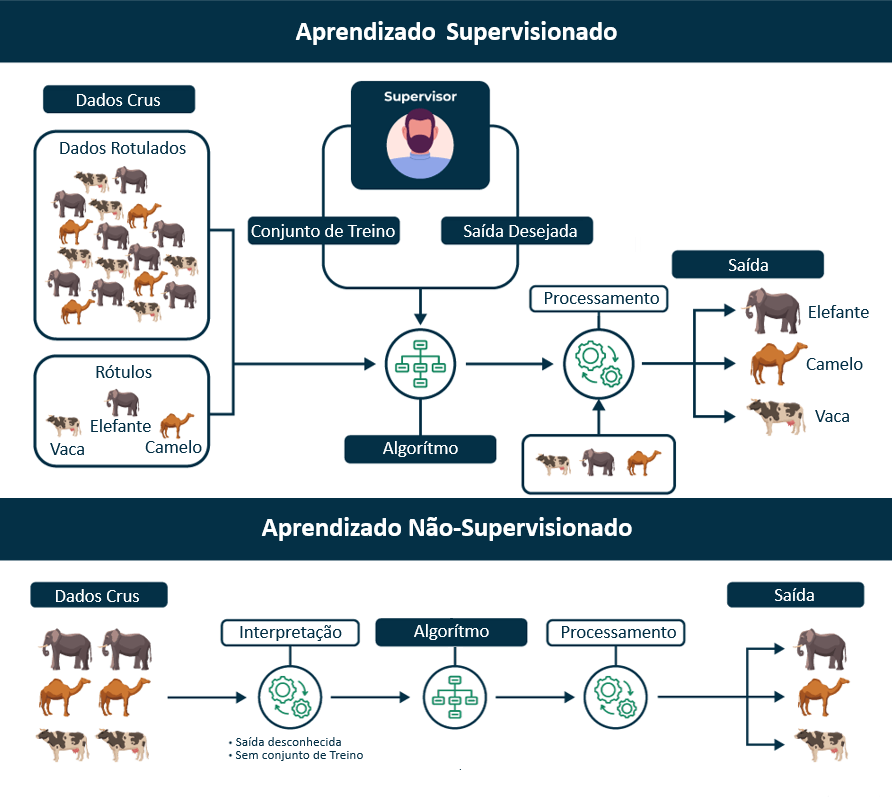
\includegraphics[width=.95\linewidth]{learning_comparison.png}
    \caption{Comparativo entre as abordagens de aprendizado de máquina. Na abordagem não-supervisionada os animais são agrupados automaticamente conforme a similaridade de suas características visuais. Já na abordagem supervisionada, destaca-se a presença de um agente supervisor, responsável por fornecer ao sistema um gabarito como base para o reconhecimento de padrões entre as associações explícitas de entrada e saída. Fonte: Adaptado de \cite{moritz2024}.}
    \label{fig:Fig_aprendizado}
\end{figure}

A literatura apresenta uma ampla variedade de técnicas supervisionadas para problemas de classificação e regressão. Entre os métodos clássicos, destacam-se: Regressão Logística, Árvores de Decisão e \textit{Support Vector Machines} (\acs{SVM}). Os detalhes técnicos dos métodos citados previamente podem ser consultados no capítulo 2 do livro \textit{Machine Learning for Brain Disorders} \cite{faouzi2023} ou, de forma mais abrangente no livro \textit{The Elements of Statistical Learning} \cite{hastie2009}. 

Entre os modelos mais avançados, destacam-se principalmente as técnicas baseadas em redes neurais, cujo principal diferencial está na automatização do processo de extração de características e reajuste de pesos (via \textit{backpropagation}), tornando-se especialmente úteis para a análise e classificação de dados complexos. É importante destacar que, as técnicas supervisionadas baseadas em redes neurais exigem um treinamento prévio com uma base robusta, a fim de promover o ajuste de pesos e, consequentemente a generalização.


\section{Aprendizado Baseado em Redes Neurais}

As Redes Neurais Artificiais (\acsp{RNA}) constituem uma das principais abordagens no campo do aprendizado de máquina, especialmente quando se busca modelar relações complexas em dados de alta dimensionalidade. Inspiradas no funcionamento do cérebro humano, essas redes são compostas por unidades de processamento denominadas neurônios artificiais, organizadas em camadas interconectadas, conforme ilustrado na Figura \ref{fig:ann_architecture}. Um dos principais diferenciais das \acsp{RNA} é sua capacidade em aprender representações ocultas e abstratas de forma automática, o que as torna altamente eficazes em tarefas como classificação, regressão e tomada de decisão.

\begin{figure}[h]
    \centering
    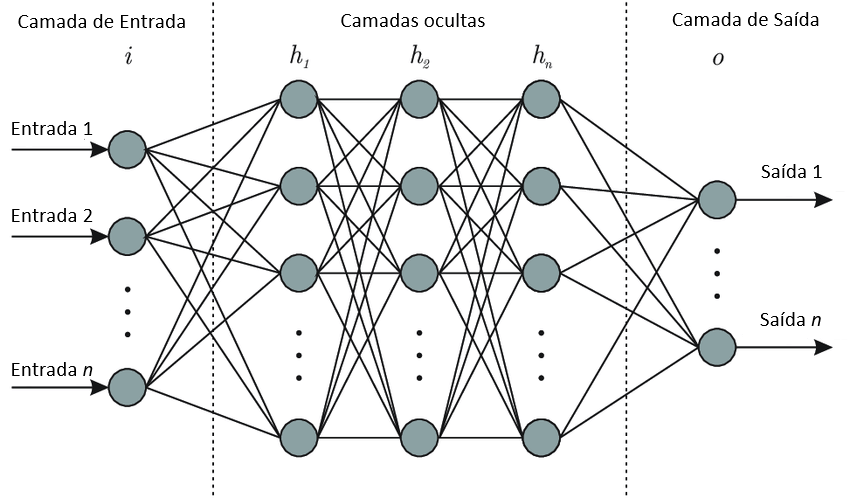
\includegraphics[width=.8\linewidth]{ann_architecture.png}
    \caption{Arquiteura de uma \acs{RNA}. Fonte: Adaptado de \cite{Alqahtani2020}.} 
    \caption*{\small A camada de entrada é responsável exclusivamente pelo transporte de dados para as camadas ocultas, as quais são responsáveis por realizar transformações mais críticas que permitem a extração de características dos dados pela rede; A camada de saída é responsável por fornecer a previsão ou o resultado do modelo.}
    
    \label{fig:ann_architecture}
\end{figure}

Os neurônios artificiais constituem as unidades básicas de processamento dessas redes. Sua função é receber entradas, processá-las por meio de operações matemáticas e produzir uma saída que será propagada para os neurônios da camada seguinte. Embora o funcionamento de um único neurônio seja relativamente simples, a organização desses elementos em múltiplas camadas interconectadas permite a modelagem de relações altamente complexas entre os dados.

À medida que a informação percorre as camadas mais profundas, os neurônios passam a atuar de forma cooperativa, identificando padrões em diferentes níveis de abstração. Em aplicações envolvendo imagens, por exemplo, as camadas iniciais tendem a aprender padrões mais simples, como bordas e texturas, enquanto camadas intermediárias e profundas capturam estruturas mais complexas, como formas, objetos ou até mesmo expressões faciais completas.

Um elemento central no funcionamento das \acsp{RNA} é o peso sináptico, que corresponde ao valor numérico associado a cada conexão entre neurônios. Esses pesos determinam a importância relativa de cada entrada no processo de decisão do neurônio e constituem os principais parâmetros ajustáveis do modelo. Durante o treinamento, os valores são atualizados iterativamente por meio do algoritmo de retropropagação (\textit{backpropagation}), no qual o cálculo dos gradientes da função de perda (loss function) é utilizado para o ajuste dos pesos definidos nas camadas anteriores, levando à minimização dos erros de predição. Para um aprofundamento técnico, recomenda-se a literatura \textit{State-of-the-art in artificial neural network applications: A survey} \cite{abiodun2018}.

As redes neurais artificiais podem ser estruturadas de acordo com os requisitos específicos de cada aplicação visando, a melhorara do desempenho, redução do custo computacional ou a adaptação do modelo a diferentes tipos de dados. Nesse contexto, o termo 'arquitetura de rede' refere-se à forma como os neurônios são organizados e conectados, incluindo aspectos como número de camadas, funções de ativação, fluxo de dados e estratégias de regularização e treinamento.

Dentre as arquiteturas clássicas, destaca-se o \textit{Multilayer Perceptron} (\acs{MLP}), considerado uma extensão do \textit{perceptron} simples. A \acs{MLP} é composta por camadas densamente conectadas (\textit{fully connected}), nas quais cada neurônio de uma camada está conectado a todos os neurônios da camada seguinte. Além disso, trata-se de uma arquitetura do tipo \textit{feedforward}, na qual a informação flui em uma única direção, da entrada até a saída, sem conexões cíclicas.

Essa arquitetura é capaz de aprender representações não lineares dos dados, sendo particularmente eficaz em tarefas envolvendo dados tabulares ou vetoriais. No entanto, seu desempenho tende a ser limitado quando aplicada a dados com estrutura espacial complexa, como imagens, uma vez que não preserva relações locais entre os elementos de entrada. Nesse contexto, as \acsp{MLP} desempenham um papel fundamental como base para o desenvolvimento de arquiteturas mais profundas, como as Redes Neurais Densas (\acsp{DNN}), conforme ilustrado na Figura \ref{fig:dnn_vs_mlp}.

\begin{figure}[h]
	\centering
	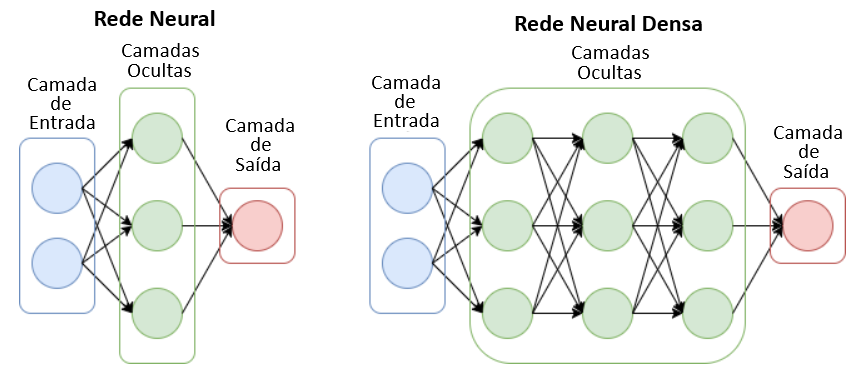
\includegraphics[width=.9\linewidth]{dnn_vs_mlp.png}
	\caption{Comparativo estrutural entre \acs{MLP} e \acs{DNN}. As redes densas mantêm a estrutura das \acsp{MLP}, porém ampliam sua profundidade por meio da adição de múltiplas camadas ocultas, o que aumenta significativamente sua capacidade de representação e abstração. Fonte: Adaptado de \cite{Wehbe2020}.}
	\label{fig:dnn_vs_mlp}
\end{figure}

A evolução das \acsp{MLP} para arquiteturas mais profundas evidencia o potencial das redes neurais em lidar com problemas cada vez mais complexos. Embora inicialmente desenvolvidas para dados vetoriais, as \acsp{DNN} demonstraram capacidade de adaptação a diferentes domínios, incluindo dados de alta dimensionalidade, como imagens, desde que adequadamente representados.

Tal processo evolutivo destaca a flexibilidade das redes neurais artificiais, cuja estrutura pode ser ajustada conforme a natureza do problema e o tipo de dado disponível. Essa característica foi essencial viabilizar o surgimento de arquiteturas mais especializadas, como as Redes Neurais Convolucionais (\acsp{CNN}) e os \textit{Vision Transformers} (\acsp{VIT}) no campo de visão computacional.

\section{Visão Computacional}

A visão computacional é um campo da inteligência artificial dedicado ao processamento e à interpretação de informações visuais provenientes do mundo real. Seu objetivo central é permitir que sistemas computacionais adquiram, analisem e interpretem imagens ou vídeos, executando tarefas que tradicionalmente dependiam da interpretação manual. Uma aplicação em visão computacional geralmente envolve um conjunto de etapas fundamentais, responsáveis por converter informações visuais em representações interpretáveis, sendo:
\begin{itemize}

    \item \textbf{Aquisição da imagem:} corresponde à captura da imagem ou vídeo por meio de dispositivos como câmeras digitais, microscópios ou sensores, responsáveis por digitalizar a cena e convertê-la em uma matriz de \textit{pixels} processável;
    
    \item \textbf{Pré-processamento:} etapa em que são aplicadas técnicas de processamento digital de imagens (\acs{PDI}), como filtragem, redimensionamento, normalização e realce de contraste, com o objetivo de melhorar a qualidade da imagem ou adequá-la às exigências do modelo;
    
    \item \textbf{Extração de características:} consiste na identificação de padrões relevantes para a análise, como bordas, contornos, texturas e formas geométricas;
    
    \item \textbf{Análise, classificação e interpretação:} etapa final, na qual técnicas de aprendizado de máquina são empregadas para classificar, segmentar ou reconhecer padrões visuais a partir das características extraídas. 
    
\end{itemize} 

O avanço neste setor está fortemente associada à evolução das redes neurais convolucionais, especialmente no que se refere à automatização da extração de características relevantes nos dados, possibilitando o desenvolvimento de modelos capazes reduzir significativamente a dependência da interpretação humana. Para um aprofundamento teórico, recomenda-se a obra \textit{Computer Vision: Algorithms and Applications} \cite{szeliski2010}.

Nesse contexto, as \acsp{CNN} utilizam filtros convolucionais para extrair automaticamente representações hierárquicas e progressivamente mais abstratas das imagens. Mais recentemente, arquiteturas baseadas nos mecanismos de atenção -- como os \acsp{VIT} -- passaram a ganhar destaque. Inspirados em modelos originalmente desenvolvidos para o processamento de linguagem natural, os \acsp{VIT} tratam imagens como sequências de fragmentos (\textit{patches}), permitindo capturar relações globais entre diferentes regiões da imagem de forma mais eficiente.

O uso de arquiteturas como \acsp{CNN} e \acsp{VIT} representam um marco na transição de abordagens baseadas em engenharia manual de características para modelos de aprendizado automático, mais escaláveis e adaptáveis, contribuíndo significativamente para o desempenho em tarefas de análise visual. Para uma visão mais abrangente sobre essas abordagens, recomenda-se a literatura \textit{A Comprehensive Survey of Deep Learning Approaches in Image Processing} \cite{trigka2025}.

\subsection{Redes Neurais Convolucionais}

As Redes Neurais Convolucionais (\acsp{CNN}) constituem uma arquitetura de aprendizado profundo projetada especificamente para lidar com dados que possuem estrutura espacial, utilizando de operações convolucionais para extrair automaticamente características hierárquicas. Adicionalmente,as \acsp{CNN} são fundamentadas em dois princípios-chave: o compartilhamento de pesos e a organização hierárquica das camadas, conforme ilustrado na Figura \ref{fig:conv_layers}.

O compartilhamento de pesos consiste na aplicação de um mesmo filtro convolucional em diferentes regiões da imagem, o que reduz significativamente o número de parâmetros do modelo e melhora sua eficiência computacional. Já a organização hierárquica das camadas permite que a rede aprenda representações progressivamente mais abstratas, partindo de padrões simples, como bordas, até estruturas mais complexas, como objetos ou regiões semânticas.

\begin{figure}[h]
    \centering
    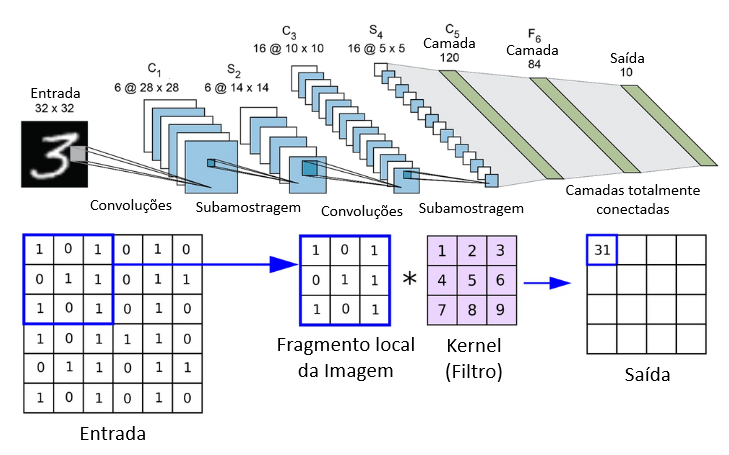
\includegraphics[width=1\linewidth]{conv_layers.png}
    \caption{Organização estrutural das camadas convolucionais em uma \acs{CNN}. O processo de convolução entre os filtros e as regiões locais da imagem permite a extração de padrões espaciais. À medida que a profundidade da rede aumenta, as representações tornam-se mais abstratas e informativas. Fonte: Adaptado de \cite{Jiang2024}.}
    \label{fig:conv_layers}
\end{figure}

A arquitetura de uma \acs{CNN} é composta por diferentes tipos de camadas, as quais são responsáveis por desempenhar uma função específica no processo de extração e interpretação das características visuais:

\begin{itemize}
    
    \item \textbf{Camada convolucional (\textit{convolutional layer}):} responsável pela aplicação de filtros (\textit{kernels}), representados por pequenas matrizes de pesos (geralmente de dimensões 3×3 ou 5×5), sobre a imagem de entrada. Durante o processo de convolução, esses filtros percorrem a imagem realizando operações locais de multiplicação e soma, das quais resultam mapas de características (\textit{feature maps}) que destacam padrões específicos presentes nos dados. Cada filtro tende a responder a determinadas características, como bordas, texturas ou formas elementares, e a utilização conjunta de múltiplos filtros permite a extração de representações cada vez mais informativas da imagem;
    
    \item \textbf{Camada de ativação:} introduz não linearidade ao modelo por meio de funções de ativação, permitindo que a rede aprenda relações complexas entre os dados. Sem essa etapa, a rede seria limitada a transformações lineares. Funções como \textit{\acs{ReLU}}, \textit{Sigmoid} e \textit{Tanh} são comumente utilizadas nesse contexto;
    
    \item \textbf{Camada de \textit{pooling} (subamostragem):} tem como objetivo reduzir as dimensões espaciais dos mapas de características, preservando as informações mais relevantes. Essa redução contribui para a diminuição do custo computacional e para a maior robustez do modelo a pequenas variações espaciais, como deslocamentos ou deformações;
    
    \item \textbf{Camadas totalmente conectadas (\textit{fully connected layers}):} nesta etapa, os mapas de características são convertidos em um vetor unidimensional por meio do processo de \textit{flattening}. Esse vetor é então utilizado como entrada para camadas densas, responsáveis por combinar as características extraídas e realizar a predição final, geralmente por meio de uma função de ativação como a \textit{softmax}, em problemas de classificação.

\end{itemize}

As \acsp{CNN} não seguem uma estrutura fixa, podendo ser adaptadas em termos de profundidade, número de filtros, tamanho dos \textit{kernels} e estratégias de conexão entre camadas. Essa flexibilidade arquitetural é uma de suas principais vantagens, permitindo sua aplicação em uma ampla variedade de problemas, desde tarefas simples de classificação até aplicações complexas em visão computacional.

Arquiteturas clássicas como \textit{AlexNet}, \textit{\acs{VGG}Net} e \textit{Inception} demonstram como diferentes estratégias de projeto podem impactar diretamente o desempenho e a escalabilidade dos modelos. Para um aprofundamento nos aspectos técnicos e nas variações arquiteturais das \acsp{CNN}, recomenda-se a literatura \textit{A review of convolutional neural networks in computer vision} \cite{zhao2024}. No contexto deste trabalho, arquiteturas convolucionais distintas foram exploradas para o problema de classificação proposto, com o objetivo de comparar seus desempenhos e identificar o modelo mais adequado para a condução dos experimentos finais.

\subsubsection*{Residual Network - ResNet}

A arquitetura \textit{ResNet} foi proposta com o objetivo de superar limitações observadas em \acsp{CNN} profundas, especialmente o problema do desaparecimento do gradiente (\textit{vanishing gradient}) e a degradação do desempenho à medida que a profundidade da rede aumenta. Em arquiteturas convencionais, o acréscimo de camadas pode dificultar o processo de otimização, resultando em piora da acurácia e instabilidade durante o treinamento, mesmo na ausência de \textit{overfitting}.

Neste contexto, a \textit{ResNet} introduz o conceito de aprendizado residual, o qual é implementado por meio dos chamados blocos residuais, que incorporam conexões de atalho (\textit{skip connections}) entre camadas. Em vez de aprender diretamente a transformação desejada, o modelo passa a aprender uma função residual — isto é, a diferença entre a entrada e a saída esperada. A saída do bloco é então obtida pela soma entre essa transformação e a entrada original.

Essa estratégia favorece a propagação do fluxo de informação e do gradiente ao longo da rede, reduzindo significativamente os efeitos do desaparecimento do gradiente e facilitando o processo de otimização geral. Além disso, as conexões residuais permitem que a rede preserve informações de camadas anteriores e, quando necessário, propague a entrada sem modificações relevantes, contribuindo para maior estabilidade e desempenho em redes profundas.

De forma geral, as arquiteturas da família \textit{ResNet} são organizadas em três componentes principais: o \textit{stem}, o \textit{backbone} e o \textit{head}. O \textit{stem} corresponde ao estágio inicial da rede, responsável por realizar as primeiras operações de extração de características a partir da imagem de entrada. Tipicamente, essa etapa inclui uma convolução inicial (frequentemente com filtros 7×7 e \textit{stride} 2), seguida por normalização em lote (\textit{Batch Normalization}), função de ativação \textit{\acs{ReLU}} e uma operação de \textit{pooling}. 

Os blocos residuais, por sua vez, constituem o núcleo da arquitetura. Existem dois tipos principais de blocos na família \textit{ResNet}: o bloco básico (\textit{basic block}), utilizado em redes mais rasas (como ResNet-18 e ResNet-34), e o bloco de gargalo (\textit{bottleneck}), empregado em redes mais profundas (como ResNet-50 e superiores). O \textit{basic block} é composto por duas camadas convolucionais $3\times3$, enquanto o bloco \textit{bottleneck} utiliza uma sequência de três convoluções ($1\times1$, $3\times3$, $1\times1$), com o objetivo de reduzir e posteriormente restaurar a dimensionalidade dos canais, tornando o modelo mais eficiente computacionalmente. Em ambos os casos, a saída do bloco é somada à entrada por meio de uma conexão residual.

Os blocos são organizados em estágios (conv2\_x, conv3\_x, conv4\_x e conv5\_x), nos quais a profundidade e o número de filtros aumentam progressivamente, permitindo a extração de representações cada vez mais abstratas. Por fim, a camada final (\textit{head}) é responsável pela etapa de classificação, na qual aplica-se uma operação de \textit{Global Average Pooling} a fim de reduzir cada mapa de características a um único valor, seguida por uma camada totalmente conectada para geração das predições finais. Nesta etapa, o funcionamento ocorre de modo análogo a uma \acs{DNN}, cumprindo o papel classificatório.

Embora variantes específicas — como \textit{ResNet}-18, \textit{ResNet}-34, \textit{ResNet}-50, \textit{ResNet}-101 e \textit{ResNet}-152 — diferenciem-se principalmente pela profundidade e pelo tipo de bloco utilizado, sua estrutura conceitual permanece consistente, permitindo a adaptação da arquitetura a diferentes cenários sem comprometer a filosofia de funcionamento. Como exemplo, a Figura \ref{fig:resnet50} ilustra a construção estrutural do modelo \textit{ResNet}-50, composto por 50 camadas treináveis organizadas nos estágios \textit{stem}, \textit{bottleneck} (conv2\_x,conv3\_x, conv4\_x, conv5\_x) e \textit{head}.

\begin{figure}[h]
    \centering
    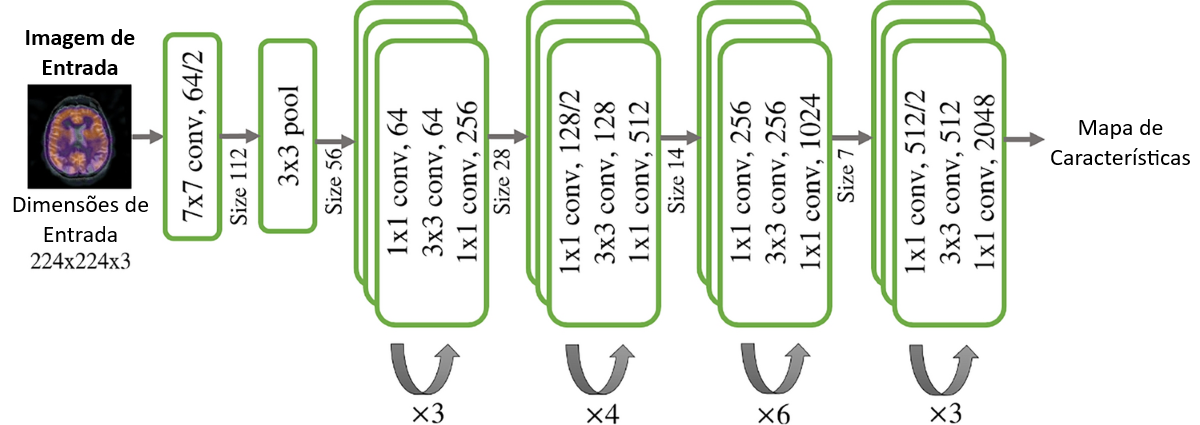
\includegraphics[width=1\linewidth]{resnet_50.png}
    \caption{Organização estrutural das camadas convolucionais no modelo \textit{ResNet50}. Fonte: Adaptado de \cite{Stack2025}.}
    \label{fig:resnet50}
\end{figure}

A arquitetura \textit{ResNet} teve um impacto significativo no avanço do aprendizado profundo, ao viabilizar o treinamento de redes com dezenas ou até centenas de camadas de forma estável. Sua proposta de aprendizado residual tornou-se um marco na área, influenciando o desenvolvimento de diversas extensões, como a \textit{ResNeXt}, que introduz o conceito de cardinalidade (múltiplos caminhos paralelos dentro dos blocos), a \textit{Wide ResNet}, que prioriza o aumento da largura da rede, e a \textit{ResNetV2}, que modifica a ordem das operações internas para melhorar a estabilidade do treinamento.  A estrutura descrita previamente, bem como a topologia padrão da arquiteura podem ser consultadas com maior detalhamento por meio do artigo \textit{Deep Residual Learning for Image Recognition} \cite{he2016}.

\subsubsection*{Densely Connected Convolutional Network - DenseNet}

A \textit{DenseNet} introduz um padrão de conectividade distinto no contexto das \acsp{CNN}, no qual cada camada recebe como entrada os mapas de características de todas as camadas anteriores dentro de um mesmo bloco \cite{Huang2017}, conforme ilustrado pela Figura \ref{fig:densenet_str}. Como consequência, cada camada tem acesso direto tanto a informações de baixo nível (como bordas e texturas) quanto a representações mais abstratas, aprendidas em camadas mais profundas. 

\begin{figure}[h]
	\centering
	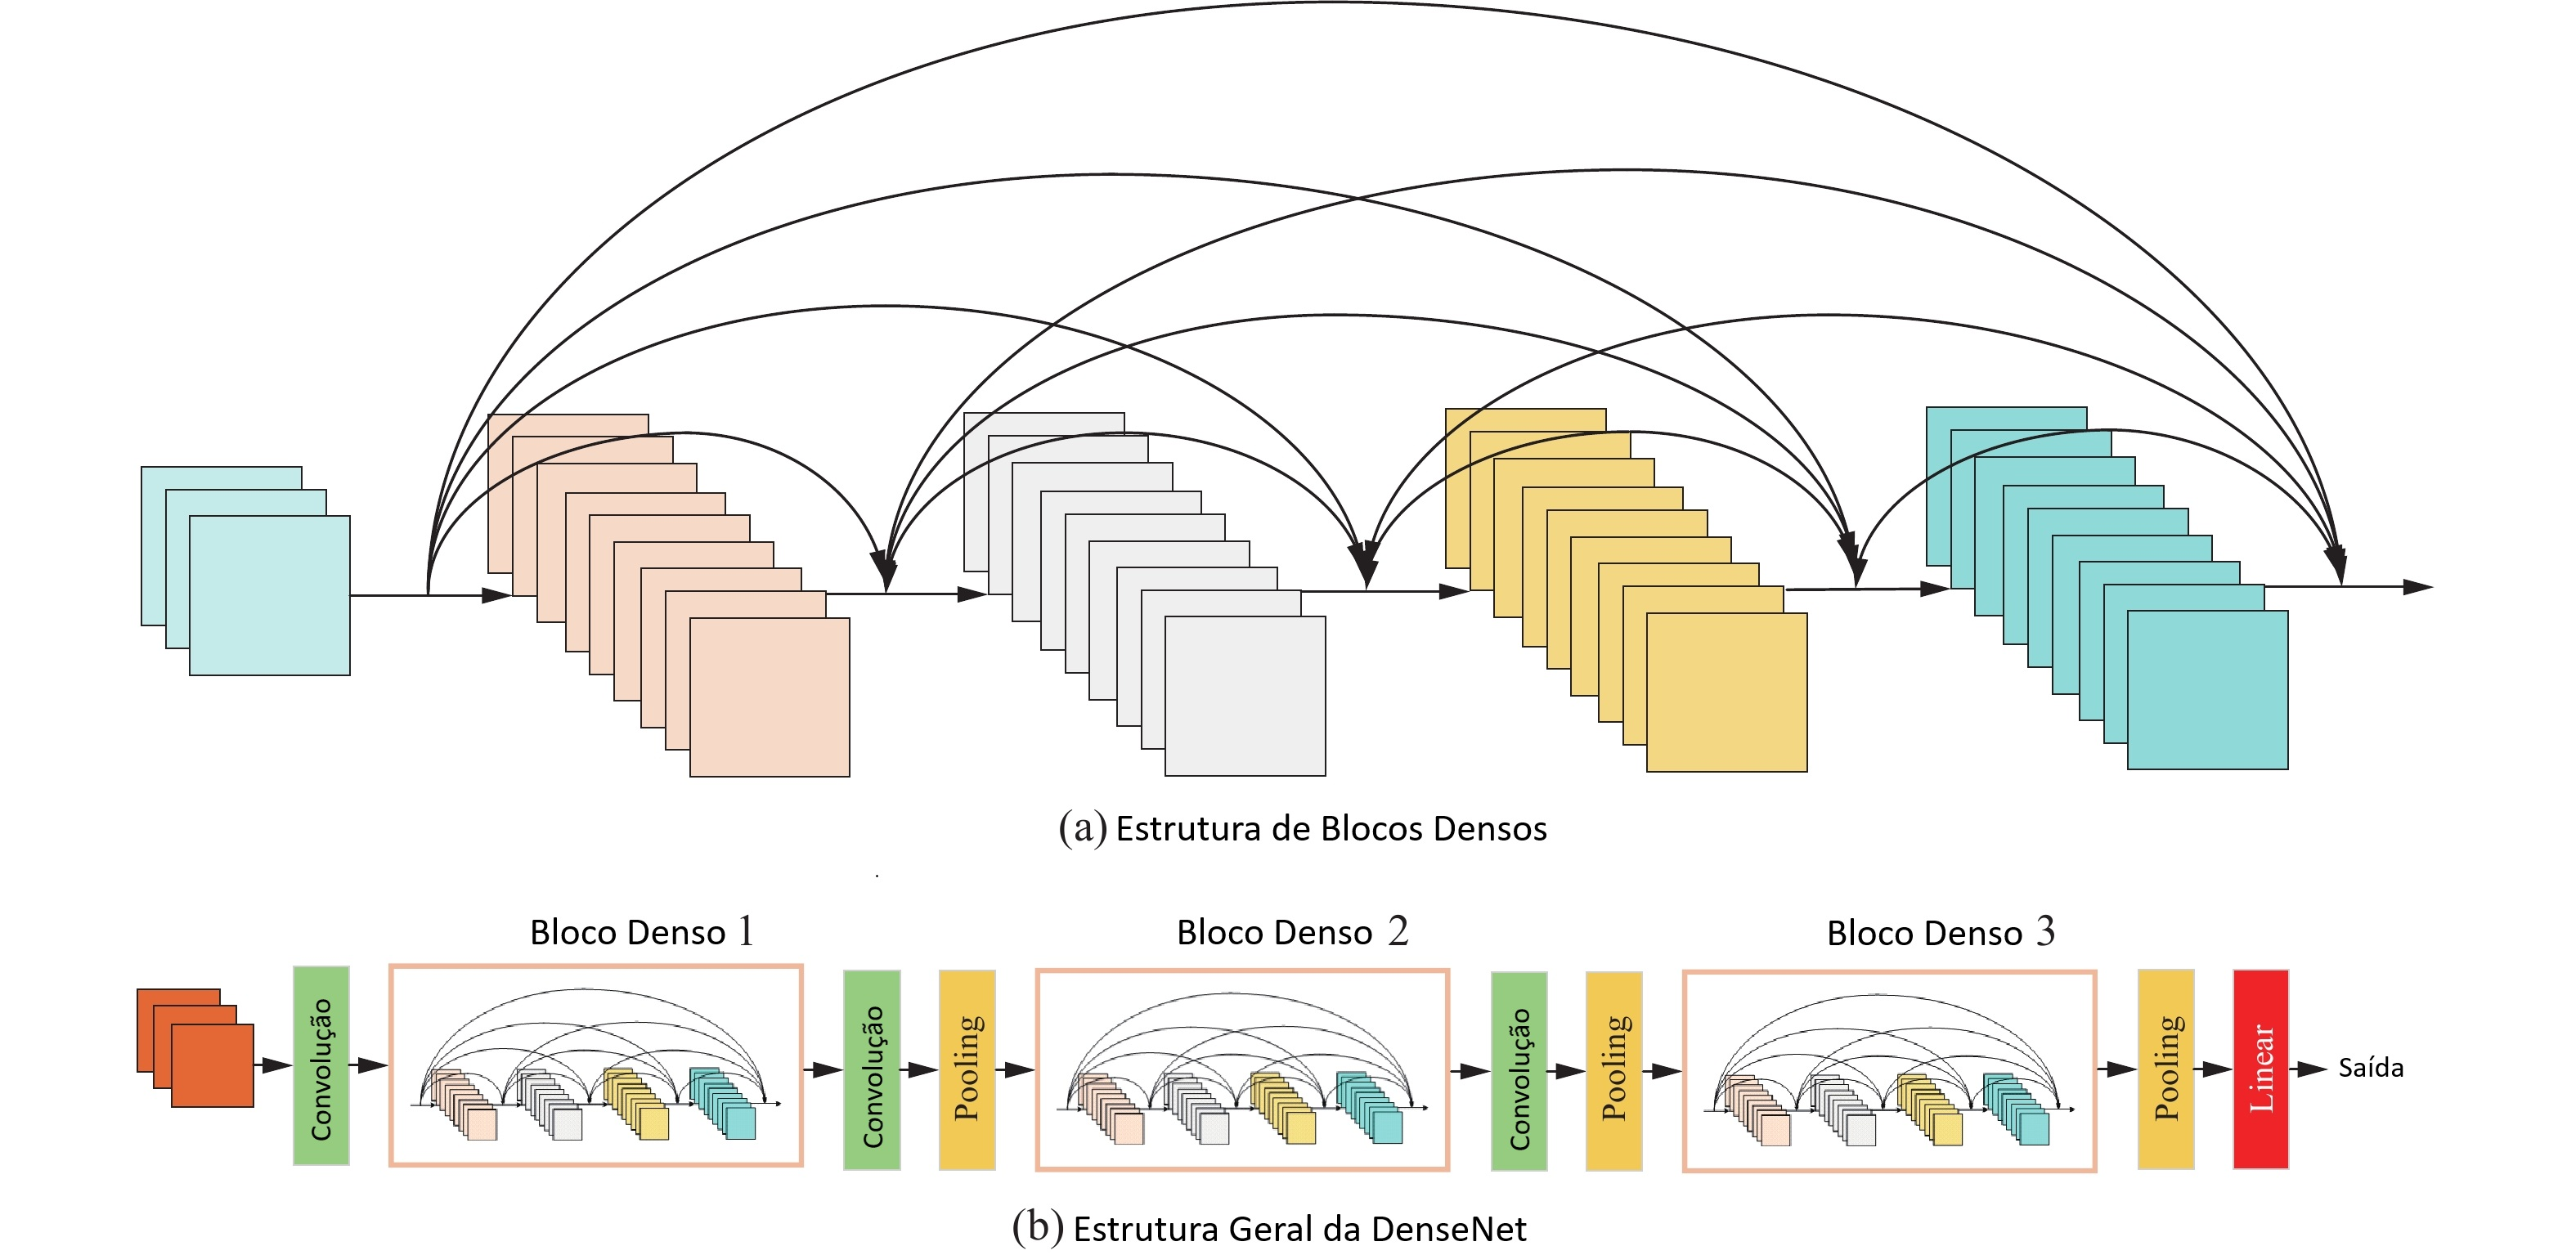
\includegraphics[width=0.9\linewidth]{figuras/figs_fundamentacao/DenseNet_Str}
	\caption{Estrutura da arquitetura \textit{DenseNet}, com destaque para o reaproveitamento completo de características entre as camadas. Fonte: Adaptado de \cite{jia2021cnn_palmprint}.}
	\label{fig:densenet_str}
\end{figure}

Diferentemente das \acsp{CNN} tradicionais, em que a informação flui de forma sequencial entre camadas adjacentes, a \textit{DenseNet} promove um fluxo de informação mais intenso e contínuo ao longo da rede, favorecendo um alto reaproveitamento de características e  contrastando diretamente com a abordagem adotada pela \textit{ResNet}, na qual as conexões residuais realizam somas entre entradas e saídas de blocos. Formalmente, considerando um bloco denso com $L$ camadas, a entrada da camada $l$ ($x_l$) é definida como a concatenação $H_l(\cdot\cdot\cdot)$ das saídas de todas as camadas anteriores, conforme descrito pela equação \ref{eq:denset_concat}. 

\begin{equation}
	\begin{aligned}
		\displaystyle x_l &= H_l([x_0, x_1, x_2, \dots, x_{l-1}]) \\[8pt]
		&\text{onde:} \\
		&x_l \rightarrow \text{entrada da camada } l \\
		&H_l \rightarrow \text{operação de concatenação das saídas anteriores}
	\end{aligned}
	\label{eq:denset_concat}
\end{equation}

Do ponto de vista estrutural, a DenseNet é organizada em blocos densos (\textit{dense blocks}), intercalados por camadas de transição (\textit{transition layers}). Dentro de cada bloco denso, múltiplas camadas convolucionais são empilhadas com conexões completas entre si. Já as camadas de transição são responsáveis por controlar o crescimento do número de canais e reduzir a dimensionalidade espacial dos mapas de características, sendo geralmente compostas por convoluções $1\times1$ seguidas de operações de \textit{pooling}.

Um conceito central na \textit{DenseNet} é a taxa de crescimento (\textit{growth rate}), que define quantos novos mapas de características cada camada adiciona ao conjunto global. Diferentemente de arquiteturas convencionais, em que o número de filtros pode crescer rapidamente, a \textit{DenseNet} mantém esse crescimento controlado, o que contribui para a eficiência do modelo em termos de número de parâmetros. 

A conectividade densa favorece a propagação do gradiente ao longo da rede, mitigando problemas como o desaparecimento do gradiente (\textit{vanishing gradient}), de maneira semelhante — porém estruturalmente distinta — à estratégia adotada pela ResNet. Além disso, o forte reaproveitamento de características reduz a necessidade de aprender representações redundantes, resultando em modelos mais compactos e eficientes.

No contexto deste trabalho, a \textit{DenseNet} foi incluída como uma alternativa arquitetural à ResNet, com o objetivo de investigar o impacto na priorização do reaproveitamento explícito de características, frente ao aprendizado residual oferecido pela \textit{ResNet}. Considerando o tamanho reduzido do conjunto de dados e a natureza sutil das variações faciais associadas à dor, a capacidade da DenseNet de preservar características de baixo nível ao longo de toda a rede pode favorecer a identificação de padrões finos, potencialmente contribuindo para uma melhor generalização.

\subsubsection*{Mobile Network - MobileNet}

A \textit{MobileNet} é uma arquitetura de rede neural convolucional leve, proposta por Howard et al. \cite{Howard2017}, com o objetivo de oferecer alta eficiência computacional em cenários com restrições de recursos, como dispositivos móveis e sistemas embarcados. Diferentemente de arquiteturas convencionais, que priorizam desempenho máximo mesmo à custa de alto custo computacional, a \textit{MobileNet} foi projetada com foco no equilíbrio entre acurácia e eficiência.

O principal diferencial da MobileNet está no uso de convoluções separáveis em profundidade (\textit{depthwise separable convolutions}), uma fatoração da convolução padrão que reduz significativamente o número de parâmetros e operações necessárias, conforme ilustrado pela Figura \ref{fig:mobilenetstr}. Em uma convolução tradicional, cada filtro atua simultaneamente sobre todas as dimensões espaciais e canais de entrada. Já na abordagem separável, essa operação é decomposta em duas etapas: uma convolução em profundidade (\textit{depthwise convolution}), que aplica um único filtro por canal de entrada, seguida por uma convolução ponto a ponto (\textit{pointwise convolution}, $1\times1$), responsável por combinar as informações entre os canais.

Enquanto uma convolução padrão possui custo proporcional a $D_k \times D_k \times M \times N$, sendo $D_k$ é o tamanho do kernel, $M$ o número de canais de entrada e $N$ o número de filtros, a convolução separável reduz esse custo para aproximadamente $D_k \times D_k \times M + M \times N$, resultando em uma economia significativa, especialmente em redes profundas.

\begin{figure}[h]
	\centering
	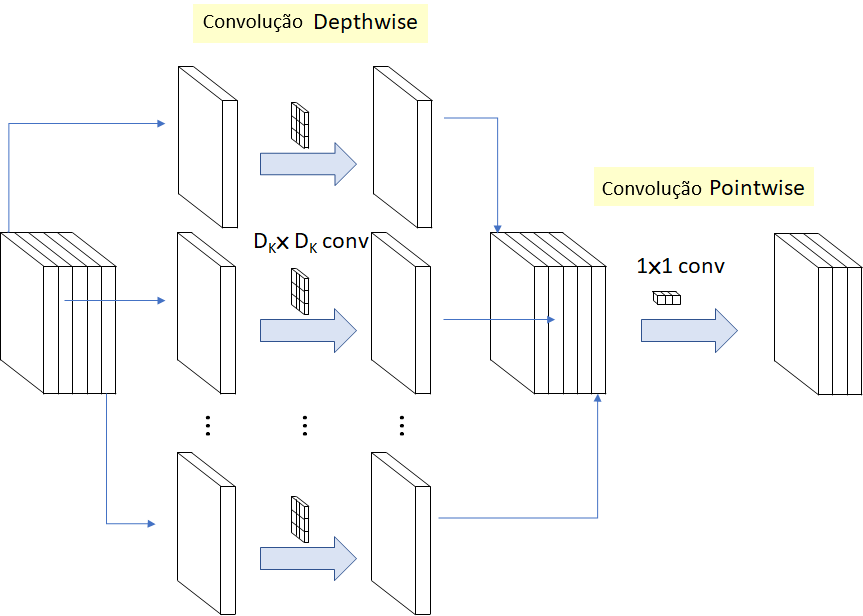
\includegraphics[width=0.7\linewidth]{figuras/figs_fundamentacao/MobileNet_str}
	\caption{Estrutura convolucional adotado pela \textit{MobileNet}, baseada em operações separáveis em profundidade. Fonte: Adaptado de \cite{tomar2021crowd}.}
	\label{fig:mobilenetstr}
\end{figure}

Adicionalmente, a \textit{MobileNet} introduz dois hiperparâmetros importantes que permitem ajustar o modelo conforme as restrições do problema: o multiplicador de largura (\textit{width multiplier}), que reduz proporcionalmente o número de canais em cada camada, e o multiplicador de resolução (\textit{resolution multiplier}), que diminui o tamanho espacial das imagens de entrada. Esses mecanismos oferecem flexibilidade para adaptar o modelo a diferentes cenários, controlando diretamente o trade-off entre custo computacional e desempenho.

Do ponto de vista estrutural, a MobileNet segue um padrão sequencial de camadas convolucionais separáveis, intercaladas com normalização em lote (\textit{Batch Normalization}) e funções de ativação não lineares, como a \textit{\acs{ReLU}}, conforme descrito pela tabela \ref{tab:mobilenet_str}. Diferentemente de arquiteturas como a \textit{ResNet} e a \textit{DenseNet}, a MobileNet não utiliza conexões residuais densas ou estratégias explícitas de reaproveitamento de características, priorizando uma arquitetura mais simples e eficiente.


\begin{table}[h]
	\centering
	\caption{Configuração estrutural do modelo MobileNet-V1, utilizado neste estudo.}
	\label{tab:mobilenet_str}
	\renewcommand{\arraystretch}{1.3}
	
	\begin{tabular}{l|l}
		\toprule
		\textbf{Camada} & \textbf{Estrutura} \\
		\midrule
		
		Conv1 & $3 \times 3$, 32, stride 2 \\        
		Conv2 (DW + PW) & Depthwise $3 \times 3$, stride 1 + Pointwise $1 \times 1$, 64 \\        
		Conv3 (DW + PW) & Depthwise $3 \times 3$, stride 2 + Pointwise $1 \times 1$, 128 \\        
		Conv4 (DW + PW) & Depthwise $3 \times 3$, stride 1 + Pointwise $1 \times 1$, 128 \\        
		Conv5 (DW + PW) & Depthwise $3 \times 3$, stride 2 + Pointwise $1 \times 1$, 256 \\
		Conv6 (DW + PW) & Depthwise $3 \times 3$, stride 1 + Pointwise $1 \times 1$, 256 \\
		Conv7 (DW + PW) & Depthwise $3 \times 3$, stride 2 + Pointwise $1 \times 1$, 512 \\
		
		Conv8--12 ($\times 5$) 
		& \makecell[l]{
			Depthwise $3 \times 3$, stride 1 \\
			Pointwise $1 \times 1$, 512
		}\\
		
		Conv13 (DW + PW) & Depthwise $3 \times 3$, stride 2 + Pointwise $1 \times 1$, 1024 \\
		Conv14 (DW + PW) & Depthwise $3 \times 3$, stride 1 + Pointwise $1 \times 1$, 1024 \\
		
		\midrule
		
		AvgPool & Global average pooling \\ 
		Dropout & 0.3 \\
		FC & Fully connected (3 classes, softmax) \\
		
		\bottomrule
	\end{tabular}
\end{table}

A \textit{MobileNet} apresenta um contraste importante com as demais arquiteturas analisadas neste trabalho. Enquanto a \textit{ResNet} utiliza conexões residuais para facilitar o fluxo de gradientes em redes profundas, e a \textit{DenseNet} promove o reaproveitamento intensivo de características por meio de conexões densas, a MobileNet adota uma abordagem focada na eficiência estrutural, reduzindo a complexidade das operações internas da rede. 

Neste estudo, a \textit{MobileNet} foi incorporada com o objetivo de avaliar a viabilidade da implementação de sistemas automatizados para detecção de dor em ambientes com restrições de recursos computacionais, buscando ampliar o acesso às ferramentas de monitoramento para o bem-estar animal. Por fim, a comparação entre os modelos convolucionais fornece uma visão abrangente sobre o impacto de diferentes paradigmas ao problema proposto.

\subsection{Transformers e Vision Transformers}

As \textit{Vision Transformers} representam um avanço significativo no campo da visão computacional, sendo uma adaptação dos \textit{Transformers}, uma arquitetura originalmente desenvolvida no campo do Processamento de Linguagem Natural (\acs{NLP}) que se baseia no mecanismo de autoatenção (\textit{self-attention}), responsável por permitir que o modelo aprenda as relações globais entre os elementos de entrada. Diferentemente de abordagens convencionais, que processam as dependências de forma sequencial e local, os \textit{Transformers} analisam todos os elementos simultaneamente, atribuindo diferentes níveis de importância a cada um. Essa característica possibilita a modelagem de dependências de longo alcance logo no inicio do processo, além de possibilitar um alto grau de paralelização durante o treinamento — aspectos fundamentais para o sucesso da arquitetura em tarefas como tradução automática, sumarização de textos e modelos de linguagem em larga escala.

As \acsp{VIT} seguem princípios muito semelhantes aos \textit{Transformers} empregados em \acs{NLP}. Para compreender o funcionamento do mecanismo de autoatenção, é interessante observar um exemplo do contexto linguístico. Considerando a frase: 'O gato subiu na mesa para comer o peixe', é correto afirmar que nem todas as palavras possuem o mesmo peso para a interpretação do significado geral. Ao analisar o verbo 'comer', por exemplo, o modelo precisa concentrar maior atenção nas palavras 'gato' e 'peixe', pois são elas que estabelecem a relação semântica mais relevante. O mecanismo de atenção, portanto, tem como objetivo atribuir pesos diferentes a cada elemento da sequência, de acordo com sua importância contextual, produzindo os denominados scores de atenção — valores que indicam a influência relativa de cada palavra em relação às demais. Dessa forma, o modelo consegue representar com precisão as relações globais existentes na sequência analisada.

A primeira etapa do processo consiste em converter o texto não estruturado em um formato compreensível para o modelo computacional. Para isso, são aplicadas duas técnicas fundamentais: \textit{tokenização} e \textit{embeddings}. A \textit{tokenização} corresponde à decomposição do texto em unidades menores, denominadas \textit{tokens}, que podem ser palavras, subpalavras, símbolos ou até caracteres individuais. Essa etapa transforma o fluxo contínuo de texto em uma sequência discreta de elementos analisáveis. Em seguida, cada token é convertido em uma representação vetorial contínua, denominada embedding, os quais mapeiam elementos semelhantes para pontos próximos em um espaço vetorial multidimensional, permitindo que o modelo capture relações semânticas e sintáticas entre tais elementos. No exemplo anterior, os \textit{tokens} 'gato' e 'peixe' teriam vetores próximos nesse espaço, pois compartilham semelhanças semânticas (ambos representam animais). Essas representações são aprendidas automaticamente durante o treinamento do modelo.

Adicionalmente, além do significado das palavras, o \textit{Transformer} também precisa compreender a posição de cada \textit{token} na sequência, já que, diferentemente das redes recorrentes, ele não processa as entradas em ordem temporal. Para isso, o modelo utiliza os \textit{embeddings} posicionais (\textit{positional embeddings}), vetores que codificam a posição de cada token na sequência. Assim, a entrada final para o modelo é obtida pela soma do \textit{embedding} do \textit{token} com seu respectivo \textit{embedding} posicional — uma combinação que permite ao \textit{Transformer} considerar simultaneamente o conteúdo e a posição dos elementos durante o processamento nas camadas de autoatenção.

Após a etapa de formatação e codificação posicional, os vetores de entrada são submetidos ao mecanismo de autoatenção, responsável por modelar as relações internas entre os diferentes tokens da sequência. O processo tem início com a projeção de cada token em três espaços vetoriais distintos, obtidos por meio de transformações lineares aprendíveis. Tais projeções dão origem a três matrizes fundamentais: Query (Q), Key (K) e Value (V); Cada uma exerce um papel específico na construção das relações de atenção entre os elementos:

\begin{itemize}
    \item \textbf{Vetor Q (Query)} 	$\rightarrow$ Representa a 'pergunta' que um token faz ao resto da sequência - 'o que eu preciso saber do contexto agora?';
    \item \textbf{Vetor K (Key)} 	$\rightarrow$ Funciona como uma 'chave' ou 'assinatura' associada a cada \textit{token}, descrevendo o tipo de informação que ele pode oferecer aos demais - “o que eu tenho para oferecer a quem me perguntar?”;
    \item \textbf{Vetor V (Value)} $\rightarrow$ Representa o conteúdo efetivo que será transmitido ou agregado quando um \textit{token} recebe atenção, correspondendo à informação contextual que compõe a nova representação final.
\end{itemize}

De forma mais intuitiva, o mecanismo de autoatenção consiste em medir quanto cada \textit{token} deve prestar atenção aos demais. Para isso, cada \textit{query} é comparada com todas as \textit{keys} da sequência, produzindo um conjunto de pesos que indicam o grau de relevância de cada \textit{token} em relação ao outro. Esses pesos são, então, utilizados para calcular uma combinação ponderada dos \textit{values}, gerando uma nova representação contextualizada para cada elemento de entrada. Formalmente, são usadas três matrizes de projeção $W_Q$, $W_K$, $W_V$ $\in R^{dXd_k}$. Tais matrizes são parâmetros treináveis, ou seja, o modelo ajusta essas projeções durante o treinamento para que a atenção aprenda relações úteis para a tarefa. Com isso, as matrizes Q, K e V são definidas por: $Q = XW_Q$; $K = XW_K$; $V = XW_V$ (Sendo X o vetor de embeddings). 

É importante destacar que as matrizes de projeção $W_Q$, $W_K$ e $W_V$ são necessárias por permitirem que o modelo aprenda subespaços de representação especializados para diferentes propósitos: buscar informações (Q), indexar elementos relevantes (K) e retornar o conteúdo contextualizado (V). Caso o próprio vetor de embedding fosse utilizado diretamente como query, key e value, o modelo ficaria restrito a um único espaço de representação, limitando sua capacidade de capturar relações complexas entre os tokens. As projeções lineares, ampliam a expressividade do modelo ao permitir que a atenção opere sobre perspectivas distintas do mesmo dado, como aspectos sintáticos, semânticos ou posicionais. De maneira mais didática, temos:

\begin{enumerate}
    \item \textbf{Separação de responsabilidades} 	$\rightarrow$ cada matriz de projeção tem uma função específica dentro do cálculo de atenção:
    \begin{itemize}
        \item $W_Q$ transforma cada $x_i$ num vetor que expressa o que esse \textit{token} está buscando compreender no contexto (sua “pergunta”);
        \item $W_K$ transforma cada $x_j$ num vetor que expressa o que o \textit{token} $j$ oferece como informação disponível (sua “assinatura”);
        \item $W_V$ projeta o vetor de entrada para o espaço do conteúdo efetivo que será transmitido e agregado (sua “resposta”).
    \end{itemize}
    \item \textbf{Mudança de base / subespaços:} as projeções criam subespaços vetoriais onde as relações de similaridade entre \textit{queries} e \textit{keys} tornam-se significativas para a tarefa. Por exemplo, um subespaço pode capturar padrões sintáticos (como dependências entre verbos e sujeitos), enquanto outro pode capturar relações semânticas (como associações entre conceitos relacionados). Essa separação facilita o aprendizado de múltiplas dimensões de significado dentro de uma mesma sequência.
\end{enumerate}

Com a definição das matrizes $Q$ e $K$, torna-se possível calcular as pontuações de atenção (\textit{attention scores}), que quantificam o grau de compatibilidade (atenção) entre cada par de \textit{tokens}. Matematicamente, o modelo compara cada vetor \textit{query} $Q_i$ com todos os vetores \textit{key} $K_j$ da sequência, por meio de um produto escalar, resultando em uma medida de similaridade entre $Q_i$ e $K_j$:

\begin{equation}
    Score(i,j) = Q_i \cdot K^T_j
\end{equation}

O resultado dessa operação para todos os elementos gera uma matriz de pontuações de atenção, em que cada valor $Score(i,j)$ representa o quanto o \textit{token} na posição $i$ deve considerar o \textit{token} na posição $j$ ao atualizar seu próprio estado. Entretanto, esses valores ainda não são probabilidades; tratam-se apenas de medidas numéricas de similaridade, que podem variar amplamente em escala.

Para que possam ser interpretadas como pesos de atenção normalizados, aplica-se a função \textit{Softmax} sobre cada linha dessa matriz, transformando as pontuações em valores positivos entre 0 e 1 cuja soma é igual a 1 (probabilidades). Isso garante que o modelo distribua sua atenção de maneira ponderada entre todos os \textit{tokens}. Adicionalmente, antes da aplicação da \textit{Softmax}, as pontuações são divididas por $\sqrt{d_k}$, onde $d_k$ corresponde à dimensionalidade dos vetores \textit{key}. Essa normalização tem a função de evitar que os produtos escalares cresçam excessivamente com o aumento da dimensionalidade, o que poderia tornar a \textit{Softmax}  sensível a pequenas variações numéricas e, consequentemente, gerar gradientes instáveis durante o treinamento. Matematicamente, temos:

\begin{equation}
    Attention \: Weights(i,j) = Softmax (\frac{Q_i . K^T_j}{\sqrt{d_k}})
\end{equation}

\begin{center}
    De forma simplificada, podemos representá-la também como:
\end{center}

\begin{equation}
    Attention \: Weights(i,j) = Softmax (\frac{Score(i,j)}{\sqrt{d_k}})
\end{equation}

Após essa etapa, o modelo sabe, para cada palavra da sequência, quais outros elementos são mais relevantes para sua interpretação no contexto global. Como exemplo, podemos considerar os seguintes pesos atribuídos aos \textit{tokens} da frase 'O gato comeu':

\begin{itemize}
\item Atenção em “O”: 0.05
\item Atenção em “gato”: 0.45
\item Atenção em “comeu” (ela mesma): 0.70
\end{itemize}

Esses valores indicam que a palavra “comeu” concentra a maior parte de sua atenção em si mesma (caracterizando o princípio da autoatenção), mas também atribui uma atenção significativa à palavra 'gato' (0.45), reconhecendo que ela é o sujeito da ação expressa pelo verbo. Por outro lado, a palavra 'O' recebe um peso pequeno (0.05), o que indica que sua contribuição semântica para a compreensão de “comeu” é menos relevante. 

Com os pesos calculados, o modelo realiza o passo final da autoatenção: a combinação ponderada dos vetores de valor (\textit{Value}). Cada vetor $V_j$ contém a informação contextual de um \textit{token} da sequência, e o peso de atenção $Attention : Weights(i,j)$, responsável por definir quanto dessa informação deve ser incorporada ao token $i$. O resultado é obtido pela soma ponderada de todos os \textit{Values}, dada pela seguinte expressão:

\begin{equation}
    Output(i) = \sum_j Attention \: Weights(i,j) \: \times \: V_j
\end{equation}

Assim, o vetor de saída $Output(i)$ representa uma versão contextualizada do \textit{token} $i$. Ele não reflete apenas a informação original da palavra, mas também agrega, de maneira ponderada, partes das informações de todas as outras palavras que receberam atenção. No exemplo anterior, a nova representação de 'comeu' passa a carregar não apenas a ideia de uma ação, mas também a noção de quem a executa (“gato”), enriquecendo a semântica do \textit{token}. Em contraste com arquiteturas sequenciais tradicionais, o \textit{Transformer} constrói simultaneamente todas as relações de atenção, resultando em representações altamente expressivas e interconectadas.

É importante destacar que, em modelos reais, o desempenho é mais expressivo quando o sistema é capaz de examinar diferentes tipos de relações entre os elementos de entrada simultaneamente. No entanto, isso não ocorre de forma plena quando o mecanismo de autoatenção é aplicado uma única vez. Nesse caso, o modelo tende a capturar uma única perspectiva das relações entre \textit{tokens}, ou seja, uma única métrica de similaridade em um único subespaço vetorial. 

Neste contexto introduz-se o conceito de \textit{multi-head attention}, cuja ideia central é calcular múltiplos mecanismos de atenção em paralelo, cada um operando em um subespaço distinto das representações de entrada, e posteriormente combinar os resultados obtidos. De forma intuitiva, seria como observar uma mesma cena por diferentes lentes: uma lente realça as cores, outra enfatiza contornos e outra destaca texturas. Ao combinar as observações de todas essas lentes, obtém-se uma representação mais rica do que qualquer lente isolada poderia oferecer.

Matematicamente, \textit{multi-head attention} divide a projeção total em $h$ cabeças. Em vez de projetar cada embedding $X$ de dimensão $d$ diretamente nos vetores Q, K e V de dimensões $d_k$, o mecanismo cria $h$ conjunto de matrizes $W^{(i)}_Q, W^{(i)}_K, W^{(i)}_V$ que projetam para subespaços de dimensão menor (normalmente $d_k = d/h$). Para cada cabeça $i$ calcula-se a atenção, sendo:

\begin{equation}
    head_i = Attention(Q^{(i)}, K^{(i)}, V^{(i)})
\end{equation}

\begin{center}
    Onde:
\end{center}

\begin{equation}
    Q^{(i)} = XW^{(i)}_Q; K = XW^{(i)}_K; V = XW^{(i)}_V
\end{equation}

Cada uma das saídas geradas por essas cabeças resulta em uma matriz de dimensão $n \times d_k$, que representa o número de \textit{tokens} ($n$) e a dimensão de cada subespaço ($d_k$). Em seguida, todas as saídas são concatenadas para formar uma única matriz de dimensão $n \times (h \cdot d_k)$ e, por fim, projetadas novamente em um espaço de dimensão $d$ por meio de uma matriz de projeção final $W_O \in R^{(h d_k) \times d}$, obtendo-se assim a saída consolidada da camada de atenção:

\begin{equation}
    MultiHead(X) = Concat(head_1,\ldots,head_h)W_o.
\end{equation}

A arquitetura dos \textit{Transformers} é composta por blocos modulares empilhados, que combinam mecanismos de atenção com camadas \textit{feedforward}, normalização e conexões residuais. Essa estrutura caracteriza o \textit{encoder} do modelo e permite o aprendizado eficiente de dependências complexas entre os elementos da entrada. Cada camada do \textit{encoder} realiza duas operações principais, executadas em sequência:

\begin{enumerate}
    \item Uma subcamada de atenção (tipicamente a \textit{multi-head self-attention}) que permite que cada posição da sequência acesse informações provenientes de todas as demais, capturando relações globais entre os elementos;
    \item Uma subcamada \textit{feedforward} aplicada após a atenção, que executa transformações ponto a ponto de forma independente para cada posição. Entre essas subcamadas, são inseridas conexões residuais (\textit{skip connections}) e mecanismos de normalização (geralmente\textit{ Layer Normalization} ou \textit{LayerNorm}).
\end{enumerate}

A subcamada \textit{feedforward} corresponde, na prática, a uma pequena rede neural densamente conectada, aplicada individualmente a cada \textit{token}. Em geral, ela é composta por duas projeções lineares separadas por uma função de ativação não linear (como \acs{ReLU} ou \acs{GELU}). Essa etapa amplia a capacidade de modelagem local das representações: enquanto o mecanismo de atenção redistribui informações entre diferentes posições, a camada densa permite que cada posição refine e recombine suas próprias características de maneira não linear, enriquecendo a representação antes que ela seja propagada para a próxima camada.

As conexões residuais e a normalização são cruciais para viabilizar o empilhamento profundo de blocos. A conexão residual adiciona a entrada de uma subcamada à sua saída (De maneira similar à arquitetura \textit{ResNet}), o que facilita o fluxo de gradiente durante o treinamento e permite que camadas extras não degradem o desempenho. Em seguida, aplica-se a normalização, a fim de estabilizar a distribuição das ativações, melhorar a convergência e favorecer a precisão do treinamento.

Na aplicação original, a arquitetura dos \textit{Transformers} é composta por dois componentes principais: o \textit{encoder} e o \textit{decoder}. O \textit{encoder} é responsável por processar a sequência de entrada, extraindo e representando suas características em um espaço vetorial de maior expressividade. Já o \textit{decoder} utiliza essas representações para gerar uma sequência de saída, etapa essencial em tarefas como tradução automática ou geração de texto. Recomenda-se a leitura do artigo \textit{Attention Is All You Need} \cite{vaswani2017}, que apresenta em detalhes a topologia padrão dos \textit{transformers} e o funcionamento do mecanismo de atenção, sendo este, a literatura responsável por introduzir o conceito.

Nas \acsp{VIT}, o processo segue a mesma filosofia dos \textit{Transformers} originais, mas é adaptado ao domínio visual. Nesse caso, a entrada não é uma sequência de palavras, mas sim uma sequência de \textit{patches}, que representam pequenas regiões extraídas da imagem, como exemplo: em uma imagem de dimensões $224 \times 224$ \textit{pixels}, é comum dividir o conteúdo em blocos de $16 \times 16$ \textit{pixels}, o que resulta em 196 \textit{patches}. Cada um desses blocos é achatado (vetorizado) e projetado linearmente em um vetor de \textit{embedding} de dimensão fixa.

São adicionados dois elementos fundamentais à sequência de embeddings dos patches: um token de classe (\textit{class token}), que agrega a informação global da imagem e serve como representação final para tarefas de classificação, e os \textit{embeddings} posicionais, responsáveis por fornecer à rede uma noção explícita de localização espacial (Análogo ao \textit{positional encoding} das \acsp{NLP}). A sequência resultante é então processada pelo \textit{encoder} do \textit{Transformer}, cujos blocos de atenção permitem que cada patch troque informações com todos os outros, capturando dependências espaciais de longo alcance. As redes \textit{feedforward} subsequentes, por sua vez, refinam as representações locais de cada \textit{patch}, complementando a informação contextual aprendida pela atenção. Recomenda-se a leitura do artigo \textit{An Image is Worth 16x16 Words: Transformers for Image Recognition at Scale} \cite{dosovitskiy2020vit} para obter maiores detalhes técnicos acerca da construção e implementação das \acsp{VIT}, sendo esta a literatura original responsável por apresentar a técnica.

\begin{figure}[h]
    \centering
    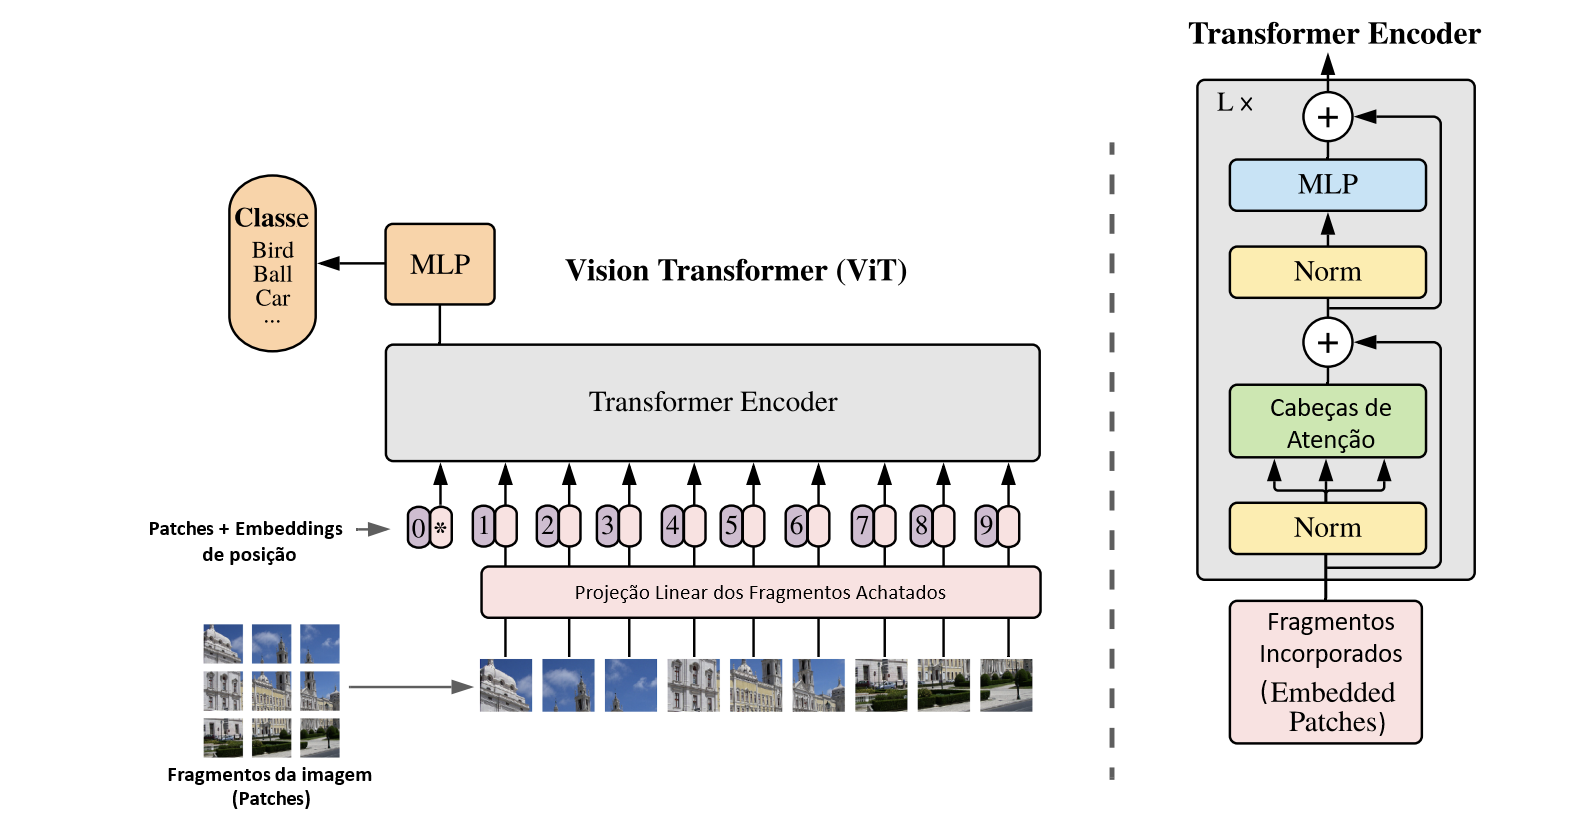
\includegraphics[width=1\linewidth]{vision_transformers.png}
    \caption{Topologia da arquiteura \textit{Vision Transformer}. Fonte: Adaptado de \cite{Huang2023}.}
    \label{fig:vit_topologia}
\end{figure}

A Figura \ref{fig:vit_topologia} ilustra de forma esquemática a topologia padrão da arquitetura \textit{Vision Transformer}, conforme descrita na literatura. A seguir, apresenta-se uma descrição intuitiva de sua estrutura, bem como a configuração de seus principais componentes e hiperparâmetros:

\begin{enumerate}

    \item \textbf{\textit{Input}:}
    \begin{itemize}
        \item A imagem de entrada possui dimensões $224\times224\times3$, correspondendo a imagens coloridas RGB (com 3 camadas) de resolução padrão;
        \item Cada imagem é dividida em \textit{patches} não sobrepostos de tamanho $16\times16$, resultando em $196$ \textit{patches} distintos;
        \item Cada \textit{patch} é achatado (\textit{flattened}) e projetado linearmente e formar o espaço de embeddings
    \end{itemize}
    
    \item \textbf{\textit{Patch Embedding} e \textit{Positional Encoding}:}
    \begin{itemize}
        \item Cada \textit{patch} é transformado por uma camada linear (projeção aprendível) que mapeia o vetor achatado de dimensão $16\times16\times3 = 768$ para um espaço de embedding de mesma dimensão ($d=768$);
        \item Um vetor adicional denominado \textit{class token} [CLS] é concatenado ao início da sequência de \textit{patches}, a fim de agregar a informação global da imagem;
        \item São adicionados embeddings posicionais aprendíveis (\textit{learnable positional embeddings}) aos vetores de entrada, preservando a informação espacial.
    \end{itemize}

    \item \textbf{\textit{Transformer Encoder}:}
    \begin{itemize}
        \item O modelo padrão \acs{VIT} é composto por 12 blocos de \textit{Transformer Encoder}, cada um contendo duas subcamadas principais: 
        \textit{(i)} \textit{Multi-Head Self-Attention} (\acs{MHSA}) e 
        \textit{(ii)} \textit{Feed-Forward Network} (\acs{FFN}), ambas com conexões residuais e normalização de camada (\textit{LayerNorm});
        \item Cada bloco utiliza 12 cabeças de atenção, cada uma com dimensão de 64, totalizando $12\times64 = 768$ dimensões, correspondendo à dimensão do embedding;
        \item A subcamada \textit{Feed-Forward} interna (\acs{MLP}) é composta por duas camadas densas com ativação não linear \acs{GELU}, sendo a primeira de dimensão $4d = 3072$ e a segunda de dimensão $d = 768$;
        \item É aplicado \textit{dropout} de 0.1 nas conexões e ativações para reduzir o risco de \textit{overfitting};
        \item O modelo é otimizado com o algoritmo \textit{AdamW}, utilizando \textit{learning rate} inicial de 0.001 e \textit{warmup} nas primeiras iterações, conforme recomendado para estabilizar o treinamento de arquiteturas baseadas em atenção.
    \end{itemize}

    \item \textbf{\textit{Class Token} e \textit{\acs{MLP} Head}:}
    \begin{itemize}
        \item Após o processamento pelos blocos do \textit{encoder}, o vetor correspondente ao \textit{class token} [CLS] é extraído como representação global da imagem;
        \item Esse vetor é passado por uma camada \textit{LayerNorm} e posteriormente por uma cabeça de classificação (\textit{\acs{MLP} Head}), composta por uma ou mais camadas densas, cuja saída é dimensionada conforme o número de classes da tarefa;
        \item A ativação final geralmente é do tipo \textit{Softmax}, produzindo uma distribuição de probabilidades sobre as classes.
    \end{itemize}

\end{enumerate}

É importante também reconhecer limitações e considerações deste tipo de arquitetura. O custo computacional do mecanismo de autoatenção cresce quadraticamente em relação ao número de \textit{patches}, o que pode tornar o treinamento inviável para imagens de alta resolução. Além disso, modelos baseados em \textit{Transformers} costumam demandar grandes volumes de dados para alcançar bom desempenho quando treinados do zero, exigindo estratégias adicionais de regularização, ajustes de taxa de aprendizado e inicialização criteriosa dos parâmetros para garantir estabilidade e convergência adequadas.

\section{Transfer Learning}

As redes neurais profundas são projetadas para aprender hierarquias de representações, em que as camadas iniciais capturam padrões visuais de baixa complexidade, como bordas e texturas, as camadas intermediárias identificam composições locais e as camadas finais abstraem conceitos de alto nível. Como muitos desses padrões de baixo e médio nível são compartilhados entre diferentes domínios visuais, o seu reaproveitamento reduz a carga de aprendizado sobre o conjunto de dados alvo. Nesse contexto, insere-se o conceito de aprendizado por transferência (\textit{Transfer Learning}).

O \textit{Transfer Learning} refere-se ao conjunto de técnicas que visam aproveitar o conhecimento adquirido por um modelo durante o treinamento em uma tarefa-fonte para melhorar o desempenho em uma tarefa-alvo, geralmente mais específica ou com menor volume de dados. A ideia central consiste em reutilizar representações previamente aprendidas (como pesos, filtros e \textit{embeddings}) provenientes de uma base de dados rica e diversa, a fim de acelerar o treinamento, reduzir a necessidade de rotulagem extensiva e aprimorar a capacidade de generalização do modelo em contextos de dados limitados.

No campo da visão computacional, o aprendizado por transferência tem se mostrado vantajoso em cenários nos quais o conjunto de dados é considerado pequeno (até 10.000 imagens) ou moderado (entre 10.000 e 100.000 imagens). Nesses casos, o esforço computacional é concentrado nas especifidades da atividade proposta, o que agiliza a convergência e evita redundâncias. No contexto deste estudo, por exemplo, a inicialização do modelo com pesos pré-treinados na base \textit{ImageNet} — um conjunto massivo composto por aproximadamente 1,2 milhão de imagens distribuídas em 1.000 categorias — permite que o processo de treinamento concentre-se na extração de características específicas e relevantes para a detecção de dor em camundongos, evitando o custo de aprendizado redundante das estruturas visuais fundamentais.

Existem duas estratégias amplamente utilizadas para a implementação do \textit{Transfer Learning}, baseadas no seguinte questionamento: “quanto do modelo original deve ser reaproveitado e quanto deve ser re-treinado?”. São elas:

\begin{enumerate}

    \item \textbf{\textit{Feature Extraction} (ou \textit{Linear Probing})}: consiste em uma abordagem mais simples e conservadora do aprendizado por transferência, na qual o modelo pré-treinado é utilizado apenas como extrator de características, sem que seus pesos internos sejam modificados. Na prática, o modelo é 'congelado', ou seja, todas as suas camadas permanecem fixas, e apenas uma nova camada final (classificadora) é adicionada e treinada. Essa camada costuma ser uma rede densa totalmente conectada com número de neurônios igual à quantidade de classes da nova tarefa.

    Como exemplo, pode-se considerar um modelo baseado na \textit{ResNet-50} pré-treinada na base \textit{ImageNet}. Nesse caso, a última camada que originalmente é responsável por classificar 1.000 categorias, é removida e substituída por uma nova camada com três saídas, adequando o modelo a uma tarefa de classificação para três classes distintas. Durante o treinamento, apenas os pesos da nova camada são atualizados, de modo que o modelo aprende apenas a interpretar as \textit{features} (características) já extraídas pelas camadas anteriores, sem modificar o processo de extração em si.

    Essa estratégia apresenta como principais vantagens o baixo custo computacional e o treinamento mais rápido, devido à menor quantidade de parâmetros ajustáveis. Entretanto, as \textit{features} aprendidas na tarefa original podem não ser totalmente adequadas à nova aplicação, o que pode limitar a capacidade de adaptação do modelo ao novo domínio.

    \item \textbf{\textit{Fine-tuning}}: trata-se de uma abordagem mais flexível, na qual parte (ou toda) a rede pré-treinada é re-treinada, permitindo o ajuste de seus pesos com base no novo conjunto de dados. A ideia é inicializar o treinamento a partir de um modelo já pré-treinado, mas, diferentemente da estratégia anterior, um subconjunto das camadas é descongelado (geralmente as últimas) para que seus pesos sejam refinados durante o processo de otimização. Dessa forma, o modelo preserva os conhecimentos gerais aprendidos (como bordas, texturas e formas), mas também passa a incorporar nuances específicas do novo domínio.

    O \textit{fine-tuning} oferece uma adaptação mais profunda ao novo domínio, permitindo ao modelo refinar suas representações internas para capturar padrões particulares da tarefa. Entretanto, o treinamento se torna computacionalmente mais caro e há maior risco de \textit{overfitting}, especialmente quando o conjunto de dados disponível é pequeno.
   
\end{enumerate}

\begin{figure}[h]
    \centering
    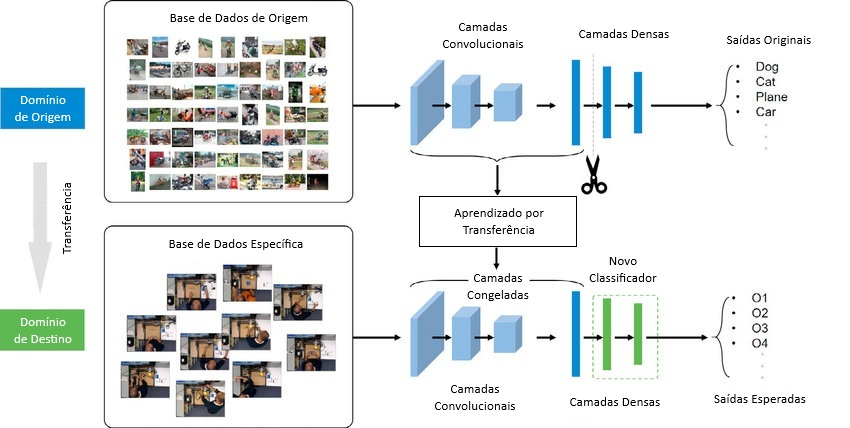
\includegraphics[width=1\linewidth]{transfer_learning_model.png}
    \caption{Exemplo intuitivo do \textit{transfer learning}, combinando o \textit{Linear Probing} com o \textit{Fine-tuning}. Fonte: Adaptado de \cite{Prabha2021}.}
    \label{fig:transfer_learning}
\end{figure}

Na prática, é comum combinar as duas estratégias descritas de forma sequencial. A Figura \ref{fig:transfer_learning} demonstra a aplicação inicial do \textit{Linear Probing} para treinar apenas a nova camada de classificação, garantindo estabilidade ao modelo. Em seguida, é feito o \textit{Fine-tuning} progressivo, no qual algumas camadas superiores são gradualmente descongeladas, e o treinamento continua com uma taxa de aprendizado reduzida. Essa abordagem é conhecida como \textit{progressive fine-tuning} ou \textit{two-stage transfer learning} e tende a produzir os melhores resultados, pois evita a instabilidade inicial de re-treinar toda a rede de uma só vez e promove uma adaptação mais controlada e eficiente ao novo domínio. Para maiores detalhes técnicos sobre a técnica de aprendizagem por transferência e as diferentes estratégias de aplicação, recomenda-se a leitura dos artigos \textit{A survey on transfer learning} \cite{pan2010},  e \textit{Fine-Tuning can Distort Pretrained Features and Underperform Out-of-Distribution} \cite{kumar2022finetuning}.

\section{TensorFlow}

Levando em consideração os objetivos deste projeto, uma ferramenta essencial para o desenvolvimento das tarefas relacionadas ao campo de inteligência artificial foi o \textit{TensorFlow}, um \textit{framework} de código aberto voltado à computação numérica e ao aprendizado de máquina, desenvolvido pelo \textit{Google}. Essa ferramenta foi projetada para expressar e executar fluxos de dados numéricos de forma eficiente e escalável. O \textit{TensorFlow} abrange tanto componentes de baixo nível, como operações tensorais, cálculo automático de gradientes e execução simbólica; quanto interfaces de alto nível, como a \acs{API} \textit{tf.keras}, que simplifica a construção e o treinamento de redes neurais.

A ideia central dessa ferramenta está na representação dos dados por meio de tensores (\textit{arrays} multidimensionais) e na descrição das operações matemáticas como nós interconectados em um grafo computacional. Esse paradigma permite que os modelos sejam definidos de maneira declarativa (especificando 'o que calcular' em vez de 'como calcular') e executados de forma paralela e otimizada em dispositivos distintos como \acs{CPU} e \acs{GPU}, sem a necessidade de alterar sua estrutura lógica. De modo geral, os tensores estão presentes em praticamente todas as etapas do processo de aprendizado, desempenhando diferentes funções dentro do fluxo de dados do modelo:

\begin{itemize}
    \item \textbf{Entradas:} os dados de entrada (imagens, textos, séries temporais) são convertidos em tensores para que possam ser processados pelas camadas subsequentes da rede;

    \item \textbf{Pesos (\textit{weights}):} cada camada da rede possui tensores treináveis, que representam os parâmetros internos (pesos e vieses) ajustados durante o processo de aprendizado;

    \item \textbf{Ativações:} os resultados intermediários (saídas produzidas por cada camada) também são tensores, os quais passam por funções de ativação (como \textit{\acs{ReLU}} ou \textit{Sigmoid}) responsáveis por introduzir não-linearidades no modelo;

    \item \textbf{Gradientes:} durante o treinamento, o \textit{TensorFlow} calcula automaticamente os tensores de gradiente, ou seja, as derivadas parciais da função de perda em relação a cada parâmetro da rede, permitindo a retropropagação do erro.
\end{itemize}

Tensores podem ser definidos como estruturas matemáticas que generalizam os conceitos de escalar, vetor e matriz para dimensões superiores. Intuitivamente, cada tensor é um \textit{array} multidimensional que armazena valores numéricos (sejam eles, inteiros, reais ou complexos) e que pode ser processado por operações matemáticas otimizadas em hardware. É importante destacar que os tensores não alteram as propriedades fundamentais das representações originais, apenas as estendem para um formato mais geral e flexível. Cada tensor é descrito essencialmente por três características principais:

\begin{enumerate}

    \item \textbf{\textit{Rank} (ordem):} indica o número de dimensões ou eixos que compõem o tensor. Essa propriedade permite compreender os tensores como extensões naturais das estruturas matemáticas básicas:


    \begin{itemize}

        \item Escalares (\textit{rank-0 tensors}) $\rightarrow$ representam um único valor numérico;

        \item Vetores (\textit{rank-1 tensors}) $\rightarrow$ representam uma sequência unidimensional de valores;
    
        \item Matrizes (\textit{rank-2 tensors}) $\rightarrow$ são usadas, para representar lotes de dados tabulares bidimensionais ou transformações lineares entre camadas;

        \item Matrizes (\textit{rank-2 tensors}) $\rightarrow$ representam dados bidimensionais, frequentemente utilizados para armazenar dados tabulares ou realizar transformações lineares entre camadas;

        \item Tensores de ordem superior (\textit{rank} $\geq$ 3) $\rightarrow$ são utilizados em domínios como visão computacional, representando imagens (3D — altura, largura e canais de cor), vídeos (4D — adicionando a dimensão temporal) e dados volumétricos (5D ou mais).

    \end{itemize}

    \item \textbf{\textit{Shape} (forma):} define o tamanho e a organização dos tensores em relação às suas dimensões. Por exemplo, um tensor com $shape = (4, 3)$ representa uma matriz composta por quatro linhas e três colunas.

    \item \textbf{Tipo de dado (\textit{dtype}):} especifica o tipo dos elementos armazenados no tensor, como \textit{float32}, \textit{int64} ou outros tipos compatíveis com o hardware de execução.

\end{enumerate}

Essas propriedades permitem que o \textit{TensorFlow} (ou qualquer outra biblioteca voltada ao \textit{deep learning}) interprete automaticamente como realizar operações entre tensores de tamanhos e tipos distintos, otimizando a alocação de memória e o paralelismo. Em sua estrutura interna, as operações sobre tensores são representadas como nós de um grafo computacional, enquanto os próprios tensores funcionam como arestas que transportam dados entre esses nós. 

Como exemplo: supondo a operação de multiplicação matricial $Z = XW + b$, os tensores $X$, $W$ e $b$ representam, respectivamente, as entradas, os pesos e o viés da transformação, resultando em um novo tensor $Z$. Durante o treinamento, cada operação armazena informações sobre o caminho computacional percorrido, permitindo ao \textit{TensorFlow} calcular automaticamente os gradientes necessários para a retropropagação do erro. Para uma descrição mais aprofundada das propriedades e operações sobre tensores, recomenda-se a consulta ao artigo de referência \textit{Tensor Decompositions and Applications} \cite{kolda2009tensor}.

O \textit{TensorFlow} disponibiliza um vasto conjunto de operações destinadas à manipulação de tensores, à execução de cálculos numéricos e ao gerenciamento de fluxos computacionais, abstraindo parte significativa da complexidade envolvida na implementação de modelos de aprendizado de máquina.Tais ferramentas tornam o \textit{framework} adequado tanto para pesquisas experimentais quanto para aplicações em larga escala, desde a etapa de prototipagem até a implantação em produção. Dentre as principais funcionalidades, destacam-se:

\begin{itemize}

    \item \textbf{Transformações estruturais:} englobam funções que permitem alterar a forma ou a organização dos tensores sem modificar seu conteúdo, possibilitando adaptações eficientes entre diferentes etapas de processamento. Entre as mais utilizadas estão: \texttt{reshape()}, \texttt{transpose()}, \texttt{concat()} e \texttt{stack()};

    \item \textbf{Operações matemáticas:} reúnem funções destinadas à realização de cálculos numéricos elementares ou compostos entre tensores, como multiplicação matricial (\texttt{matmul()}), soma (\texttt{add()}), subtração (\texttt{subtract()}), cálculo de médias (\texttt{reduce\_mean()}), entre outras;

    \item \textbf{Indexação e \textit{slicing}:} permitem acessar ou manipular regiões específicas de um tensor, de maneira análoga ao que ocorre com \textit{arrays} na biblioteca \textit{NumPy}, favorecendo o controle detalhado sobre subconjuntos de dados durante o processamento;

    \item \textbf{Broadcasting:} mecanismo que viabiliza a execução de operações entre tensores de dimensões distintas, ajustando automaticamente as dimensões de menor ordem para compatibilidade. Esse recurso é amplamente empregado em operações vetoriais e matriciais;

    \item \textbf{API para modelagem:} integra a \acs{API} \textit{Keras}, que fornece uma interface de alto nível voltada à definição, compilação e treinamento de modelos de aprendizado profundo. O \textit{Keras} padroniza a criação de camadas, funções de perda, métricas e ciclos de treinamento, além de oferecer métodos prontos para uso, como \texttt{Model.fit()} (treinamento), \texttt{Model.evaluate()} (avaliação de desempenho) e \texttt{Model.predict()} (inferência sobre novos dados), com suporte a \textit{callbacks} e registros de execução;

    \item \textbf{Otimizadores, funções de perda e métricas:} integração de algoritmos de otimização, incluindo \textit{\acs{SGD}}, \textit{Adam}, \textit{AdamW} e \textit{RMSProp}, além de funções de perda clássicas, como \textit{cross-entropy}, \textit{mean squared error (\acs{MSE})} e \textit{Huber loss}. Adicionalmente, o framework oferece métricas de desempenho como \textit{accuracy}, \textit{precision}, \textit{recall} e \textit{\acs{AUC}}, fundamentais para o acompanhamento da evolução do treinamento.
    
    \item \textbf{Distribuição e escalabilidade:} disposição de ferramentas para o treinamento distribuído, que realizam sincronização de gradientes, divisão de lotes de dados e gerenciamento de recursos computacionais, permitindo que modelos sejam treinados de forma eficiente em múltiplas \acsp{GPU}, \acsp{TPU} ou máquinas distintas, sem necessidade de alterações significativas na \acs{API};

    \item \textbf{Implantação e produção:} oferece suporte nativo à exportação e execução de modelos em diferentes ambientes, por meio de ferramentas como \textit{SavedModel} (formato padrão de exportação, preservando pesos e assinaturas de entrada/saída), \textit{TensorFlow Lite} (otimização para dispositivos móveis e embarcados) e \textit{TensorFlow.js} (execução direta em navegadores web);

    \item \textbf{Reutilização de conhecimento e monitoramento:} o \textit{Keras} também fornece acesso simplificado a modelos e pesos pré-treinados, viabilizando o uso de técnicas de \textit{transfer learning}. Adicionalmente, o \textit{TensorBoard} pode ser integrado ao processo de treinamento por meio de \textit{callbacks} e registros automáticos de \textit{logs}, permitindo a visualização de métricas, histogramas, imagens e embeddings em tempo real.

\end{itemize}

Em suma, o  \textit{TensorFlow} configura-se como uma plataforma completa voltada à pesquisa e à aplicação prática em aprendizado de máquina. Seu ecossistema abrange desde operações fundamentais sobre tensores até recursos avançados de treinamento distribuído, monitoramento e implantação de modelos em produção. Para maiores detalhes técnicos acerca das funcionalidades do \textit{Tensorflow}, recomenda-se a consulta do artigo \textit{TensorFlow: Large-Scale Machine Learning on Heterogeneous Distributed Systems} \cite{abadi2016tensorflow}.


\begin{comment}
	
	\section{Métricas para avaliação de resultados}
	
	Os resultados obtidos durante a experimentação científica exigem um processo de avaliação sólido e sistemático, de modo a verificar o comportamento e a eficácia dos modelos desenvolvidos. A aplicação de métricas e ferramentas de avaliação permitem mensurar o desempenho e a capacidade de generalização do modelo, além de reduzir o risco de interpretações imprecisas e orientar a tomada de decisões fundamentadas. 
	
	Dentre as ferramentas mais utilizadas para análise de desempenho em tarefas de classificação, destaca-se a Matriz de Confusão, uma estrutura tabular que compara as previsões realizadas pelo modelo com os valores reais das classes. Essa matriz fornece uma visão detalhada dos acertos e erros cometidos, sendo amplamente empregada para avaliar a confiabilidade e a robustez de classificadores supervisionados. A matriz é composta por quatro elementos fundamentais, que representam as possíveis combinações entre os rótulos reais e as previsões realizadas pelo modelo:
	
	\begin{itemize}
		\item \textbf{Verdadeiros positivos (\textit{True positive} - TP)}: casos rotulados como verdadeiros, que foram corretamente previstos;
		\item \textbf{Verdadeiros negativos (\textit{True Negatives} - TN)}: casos rotulados como negativos que corretamente previstos;
		\item \textbf{Falsos positivos (\textit{False Positive} - FP)}: casos negativos classificados como positivos (indica um alarme falso);
		\item \textbf{Falsos negativos (\textit{False Netgative} - FN)}: casos positivos classificados como negativos (indica uma falha de detecção do modelo).
	\end{itemize}
	
	A construção da matriz de confusão segue o princípio de que as \textbf{linhas} representam as classes reais e as \textbf{colunas} representam as classes previstas. Dessa forma, cada célula $(i, j)$ contém a quantidade de amostras cuja classe real é $i$ e que foram classificadas como pertencentes à classe $j$. Essa disposição permite identificar padrões de erro e compreender quais classes apresentam maior confusão entre si. Como exemplo, temos:
	
	\begin{table}[H]
		\centering
		\caption{Matriz de confusão ilustrativa para classificação binária}
		\label{tab:matriz_confusao}
		\renewcommand{\arraystretch}{1.8} % Aumenta o espaçamento entre linhas
		\setlength{\tabcolsep}{12pt} % Aumenta o espaçamento horizontal entre colunas
		\begin{tabular}{|c|c|c|c|}
			\hline
			\multicolumn{2}{|c|}{} & \multicolumn{2}{c|}{\textbf{Valor Predito}} \\ 
			\hline
			\multicolumn{2}{|c|}{} & \textbf{Sim} & \textbf{Não} \\ 
			\hline
			\multirow{2}{*}{\rotatebox{90}{\textbf{Real}}} 
			& \textbf{Sim} & \cellcolor{gray!20}\textbf{Verdadeiro Positivo (TP)} & \cellcolor{gray!5}\textbf{Falso Negativo (FN)} \\ 
			\cline{2-4}
			& \textbf{Não} & \cellcolor{gray!5}\textbf{Falso Positivo (FP)} & \cellcolor{gray!20}\textbf{Verdadeiro Negativo (TN)} \\ 
			\hline
		\end{tabular}
	\end{table}
	
	A partir destes valores, é possível definir as métricas básicas de avaliação (levando em consideração o problema de classificação binária). São elas:
	
	\begin{enumerate}
		\item \textbf{Acurácia (\textit{Accuracy})}: refere-se à proporção de predições corretas feitas pelo modelo. É uma métrica intuitiva, porém enganosa em classes desbalanceadas. 
		
		\begin{equation}
			Accuracy = \frac{TP+TN}{TP+TN+FP+FN};
		\end{equation}
		
		
		\item \textbf{Precisão (\textit{Precision})}: é a medida do quão confiáveis são as predições positivas do modelo, portanto, a alta precisão sugere a existência de poucos falsos positivos (alarme falso). Essa métrica responde ao seguinte questionamento: "dentre as amostras previstas como positivas, qual fração é realmente positiva?". 
		
		\begin{equation}
			Precision = \frac{TP}{TP+FP};
		\end{equation}
		
		\item \textbf{Revocação / Sensibilidade / \textit{Recall}}: refere-se à proporção de positivos reais que foram corretamente detectados, portanto, um alto \textit{recall} sugere a existência de poucos falsos negativos (falha de detecção). Essa métrica responde ao seguinte questionamento: "entre todos os positivos reais, quantos foram detectados?".
		
		\begin{equation}
			Recall = \frac{TP}{TP+FN}
		\end{equation}
		
		\item \textbf{\textit{F1-score}}:  métrica de avaliação que combina precisão e \textit{recall} em um único valor, representando um equilíbrio entre as duas métricas. É calculada como a média harmônica de precisão e \textit{recall}, sendo mais útil do que a acurácia em conjuntos de dados desequilibrados.
		
		\begin{equation}
			F1 = 2 \cdot \frac{Precision \cdot Recall}{Precision + Recall};
		\end{equation}
		
		\item \textbf{Especificidade / \textit{True Negative Rate} (TRN) }: refere-se à capacidade de um modelo identificar corretamente instâncias que pertencem à classe negativa. Essa métrica é crucial quando o custo de falsos positivos é alto, como na detecção de fraude ou na triagem de doenças.
		
		\begin{equation}
			TRN = \frac{TN}{TN+FP};
		\end{equation}
		
		\item \textbf{AUC-ROC e Curva ROC}: Curva ROC é um gráfico que exibe o desempenho de um modelo de classificação binária, plotando a Taxa de Verdadeiros Positivos (Recall) contra a Taxa de Falsos Positivos (definido por $1 - TRN (Especificidade)$) em diferentes limites de decisão. A AUC (Área sob a Curva ROC) é um valor único entre \(0\) e \(1\) que resume a performance geral do modelo, representando a probabilidade de que o modelo classifique corretamente uma instância positiva aleatória à frente de uma negativa aleatória.
		
	\end{enumerate}
	
	É importante destacar que em tarefas multiclasses, existem várias matrizes de confusão, uma para cada classe (considera-se cada classe como 'positiva' e todas as demais como 'negativas'). Dessa forma, as métricas descritas previamente são calculadas em um esquema '\textit{onde-vs-rest}' em que uma classe é confrontada com as demais. Os resultados para cada são agregados posteriormente em uma única métrica global. Neste contexto surgem as três estratégias de agregação
	
	\begin{enumerate}
		\item \textbf{\textit{Macro-average:}} é feita a média aritmética das métricas por classe, dessa forma, todas as classes são tratadas igualmente independentemente de quantos exemplos ela possua. É a abordagem ideal quando se busca avaliar o desempenho balanceado do modelo entre todas as classes, ou seja, garantir o mesmo grau de contribuição entre classes pequenas e grandes.
		
		\begin{equation}
			Precision_{macro} = \frac{1}{N}\cdot\sum_iPrecision_i 
		\end{equation}
		\textit{O exemplo acima também é válido para as demais métricas como Recall e F1-Score;}
		
		\item \textbf{\textit{Micro-average:}} trata todas as predições igualmente, somando os valores globais de verdadeiros positivos (TP), falsos positivos (FP) e falsos negativos (FN) de todas as classes antes de calcular as métricas.Dessa forma, as classes com mais exemplos tem maior influência no resultado final.
		
		\begin{equation}
			Precision_{micro} = \frac{\sum_i TP_i}{\sum_i (TP_i+FN_i)} 
		\end{equation}
		\textit{O exemplo acima também é válido para as demais métricas como Recall e F1-Score;}
		
		\item \textbf{\textit{Weighted average:}} calcula as métricas individuais por classe, mas faz a média final ponderando cada classe pela quantidade de amostras reais que ela contém ($n_i$). Trata-se de um meio-termo entre as abordagens anteriores, considerando o peso relativo de cada classe (como na \textit{micro}), mas mantendo o cálculo por classe antes da agregação (como na \textit{macro}). Dessa forma, classes maiores tem maior influência sobre o resultado, mas sem eliminar totalmente a análise das menores.
		
		\begin{equation}
			Precision_{weighted} = \frac{\sum_i (n_i \times Precision_i)}{\sum_i n_i} 
		\end{equation}
		\textit{O exemplo acima também é válido para as demais métricas como Recall e F1-Score.}
		
	\end{enumerate}
	
	Recomenda-se a leitura do artigo \textit{Evaluation Metrics in Learning Systems: A Survey} \cite{nouri2025} para obter uma descrição mais minuciosa dos métodos descritos para avaliação de resultados em aprendizado de máquina, bem como o detalhamento de outras ferramentas e técnicas que podem ser aplicadas neste contexto.
	
	\subsection{TensorBoard para a avaliação de resultados}
	
	Neste estudo, o \textit{TensorBoard} foi adotado com o propósito de facilitar a análise e o acompanhamento dos resultados ao longo do processo de aprendizado, integrando-se à etapa de avaliação dos modelos. Conceitualmente, o \textit{TensorBoard} consiste em uma ferramenta de visualização e monitoramento desenvolvida de forma integrada ao \textit{TensorFlow}, permitindo inspecionar de maneira interativa o comportamento de modelos de aprendizado de máquina durante o treinamento.
	
	Durante a execução do treinamento, a ferramenta utiliza um objeto do tipo \textit{callback} (geralmente \texttt{tf.keras.callbacks.TensorBoard}) para registrar informações relevantes sobre a execução do modelo. Tais registros são realizados periodicamente ao final de cada época ou ao término do treinamento, e incluem métricas de desempenho, tempo de execução, estrutura do grafo computacional, além de histogramas dos pesos e gradientes. Tais informações são gravadas em arquivos locais, geralmente organizados em um diretório denominado \texttt{logs}.
	
	Vale ressaltar que, em \textit{Python}, uma função de \textit{callback} é uma função passada como argumento para outra função, sendo executada em um ponto específico da execução, geralmente após a conclusão de uma tarefa. Esse mecanismo possibilita a personalização do comportamento de processos, permitindo que ações complementares sejam realizadas automaticamente conforme o andamento do programa.
	
	As informações coletadas são posteriormente interpretadas pelo \textit{TensorBoard}, que pode ser inicializado via terminal por meio do comando \texttt{tensorboard --logdir=./logs}. Uma vez iniciado, o painel torna-se acessível por meio de um navegador web (por padrão, em \textit{http://localhost:6006}), exibindo um conjunto de abas interativas que permitem a análise visual e detalhada dos resultados obtidos durante o treinamento.
	
	O \textit{TensorBoard} é modular e organiza suas funcionalidades em diferentes abas, cada uma voltada a um tipo específico de análise. Entre as principais, destacam-se as seções de escalares, grafos e distribuições, as quais se fazem presentes em maioria das aplicações de aprendizado de máquina:
	
	\begin{enumerate}
		
		\item \textbf{\textit{Scalars} (Escalares):} apresenta gráficos de métricas quantitativas registradas durante o treinamento. Dentre elas destacam-se a função de perda  (nos conjuntos de treino e validação), acurácia, taxa de aprendizado e demais métricas personalizadas como \textit{F1-Score}, precisão e revocação. A análise destas métricas são essenciais para identificar \textit{overfitting}, monitorar a convergência e comparar diferentes execuções do mesmo modelo;
		
		\item \textbf{\textit{Graphs} (Grafos Computacionais):} exibe a estrutura do modelo em forma de grafo, mostrando as conexões entre as camadas e os fluxos de dados (tensores) entre elas. Tal análise permite Verificar se o modelo foi construído corretamente e se existem camadas desconectadas ou redundantes;
		
		\item \textbf{Distribuições e Histogramas:} exibe a distribuição dos pesos e gradientes das camadas ao longo do tempo de treinamento. Tal análise permite verificar se há explosão ou desaparecimento de gradientes e como se comporta o grau de saturação dos pesos (se estão ficando muito altos ou muito baixos);
		
	\end{enumerate}
	
	É importante destacar que o \textit{TensorBoard} também dispõe de funcionalidades voltadas a análises mais específicas, como a visualização de amostras de imagens pertencentes aos conjuntos de treino, validação ou teste ao longo do processo de treinamento. É uma funcionalidade é útil em modelos de visão computacional, uma vez que permite verificar se as imagens estão sendo carregadas e pré-processadas corretamente, além de possibilitar a inspeção visual de mapas de ativação, \textit{heatmaps} e mecanismos de atenção (quando exportados como imagens). Para informações mais detalhadas, recomenda-se a consulta da página oficial da ferramenta, a qual oferece documentação e descrição técnica do completa do TensorBoard: \textit{TensorBoard: Visualization Toolkit for Machine Learning Experimentation} \cite{tensorflow2016}. 
	
	Essa ferramenta não apenas simplifica o monitoramento técnico, como também possui relevância metodológica e científica. Suas funcionalidades favorecem a análise comparativa entre diferentes arquiteturas e configurações de hiperparâmetros, melhoram a interpretação dos resultados e auxiliam na detecção de possíveis falhas ou inconsistências durante o treinamento. Tais benefícios agregam maior confiabilidade às conclusões obtidas, evidenciando que os resultados foram derivados de um processo de monitoramento sistemático, controlado e verificável.
	
\end{comment}

